\documentclass[my_thesis.tex]{subfiles}

\begin{document}

\chapter{3D magnetic equilibria}
The description of a plasma starts with a mathematical model for its equilibrium. In this chapter, we follow \citet{Freidberg2014} and introduce the ideal MHD model, and in particular its equilibrium equations. Some important properties of ideal 3D ideal MHD equilibria are discussed, and we introduce briefly the problematic of the Pfirsch-Schl\"uter diverging current singularities associated with the assumption of existence of magnetic surfaces \citep{Grad1967}. To avoid these singularities, we introduce then two restricted classes of ideal MHD equilibria, namely the Taylor state \citep{Taylor1974,Taylor1986} and the stepped-pressure equilibrium \citep{Hole2006}. Finally we discuss how these three equilibrium models can be derived by minimizing different energy functionals.

\section{Ideal MHD}
\label{section ideal mhd}
Ideal \ac{MHD} is probably the most well-known and used model to describe macroscopic plasma equilibria. It aims at describing slow phenomena on macroscopic scales. Quasi-neutrality is assumed, \textit{i.e.} $n_e=n_i=n$, where $n_e$ and $n_i$ are the electron and ion densities respectively. The plasma is modeled with a single fluid approximation, where the pressure is isotropic and defined as the sum of the ion and electron pressure, $p=p_i+p_e=2nT$, and the temperature is defined as the average of the ion and electron temperature, $T=(T_i+T_e)/2$. In addition, it is assumed that electromagnetic waves have phase velocities negligible in comparison to the speed of light, $\omega/k\ll c$, the thermal velocities of ions and electrons are non-relativistic, $v_{Ti}\ll v_{Te}\ll c$, with $v_{Ti}=(kT_i/m_i)^{1/2}$, $k$ is Boltzmann constant, and $m_i$ the ion mass. Phenomena described by ideal MHD have frequencies smaller than the electron plasma frequency, $\omega\ll \omega_{pe}=(n_ee^2/m_e\epsilon_0)^{1/2}$, where $e$ the elementary charge, $m_e$ the electron mass and $\epsilon_0$ the vacuum permittivity, and have characteristic length larger than the Debye length, $a\gg \lambda_D=(kT_e/4\pi n_e e^2)^{1/2}$. Finally, electron inertia is neglected, \textit{i.e.} their response to a force is instantaneous.

The ideal \ac{MHD} equations are \citep{Freidberg2014},
\begin{align}
	\frac{\partial \rho}{\partial t} + \nabla\cdot(\rho\mathbf{v}) &= 0 \label{mass equation}\\
	\rho\frac{d\mathbf{v}}{dt} &= \mathbf{J}\times\mathbf{B} - \nabla p \label{momentum equation}\\
	\frac{d}{dt}\left(\frac{p}{\rho^\gamma}\right) &= 0 \label{energy equation}\\
	\mathbf{E} + \mathbf{v}\times\mathbf{B} &= 0 \label{ideal Ohms law}\\
	\nabla\times\mathbf{B} &=\mu_0\mathbf{J} \label{equation ampere}\\
	\nabla\cdot\mathbf{B}&=0 \label{equation div B}\\
	\nabla\times\mathbf{E}&=-\frac{\partial \mathbf{B}}{\partial t}, \label{equation rot E}
\end{align}
where $\mathbf{J}$ and $\rho$ are the current and mass densities, $\mu_0=4\pi 10^{-7}$ is the vacuum permeability, $\mathbf{E}$ is the electric field and $\mathbf{v}$ is the fluid velocity. Note that Ampere's law, Eq.(\ref{equation ampere}), implies charge conservation,
\begin{equation}
	\nabla\cdot\mathbf{J} = 0\label{equation charge conservation}
\end{equation}

At equilibrium, all time derivatives vanish ($\partial/\partial t = 0$), and assuming zero flow ($\mathbf{v}=0$), we get the \emph{ideal MHD equilibrium equations},
\begin{align}
	\mathbf{J}\times\mathbf{B} &= \nabla p \label{equation perp force balance}\\
	\nabla\times\mathbf{B} &=\mu_0\mathbf{J}\\
	\nabla\cdot\mathbf{B}&=0.\label{equation div B ideal mhd}
\end{align}
Note that flows are damped in general magnetic equilibria, making the assumption $\mathbf{v}=0$ reasonable. Special cases are quasi-symmetric fields \citep{boozerTransportIsomorphicEquilibria1983,nuhrenbergQuasihelicallySymmetricToroidal1988,helanderTheoryPlasmaConfinement2014a,rodriguezNecessarySufficientConditions2020}, where strong flows can be generated in the direction of the symmetry \citep{spongGenerationDampingNeoclassical2005,helanderIntrinsicAmbipolarityRotation2008,simakovPlasmaRotationQuasisymmetric2011}. In tokamaks, for example, \ac{NBI} generates strong flows \citep{suckewerToroidalPlasmaRotation1979}. In this thesis, flow is neglected, as no quasi-symmetric equilibria are computed. 



% ============================================= FIGURE OF MERITS ===========================================
\subsection{Figures of merit of magnetic equilibria}
We consider a toroidal plasma volume $\mathcal{V}_P$ at equilibrium, in which the pressure $p$ and magnetic field $\mathbf{B}$ is known everywhere. We define a poloidal angle $\theta$ and a toroidal angle $\zeta$, and their corresponding basis vector $\mathbf{e}_\theta$ and $\mathbf{e}_\zeta$. We construct a radial coordinate $s$, where $s=0$ on the magnetic axis, $s=1$ at the plasma boundary, and $s=\text{const}$ on a magnetic surface. Finally, we assume that there exist a magnetic surfaces at $s=c$, parametrized by $\mathbf{x}=R(\theta,\zeta)\mathbf{e}_R + Z(\theta,\zeta)\mathbf{e}_Z$, with $(\mathbf{e}_R,\mathbf{e}_\zeta,\mathbf{e}_Z)$ the usual cylindrical unitary coordinate basis. On the magnetic surface, 
\begin{align}
	\mathbf{e}_\theta &= \frac{\partial R}{\partial \theta}\mathbf{e}_R + \frac{\partial Z}{\partial \theta}\mathbf{e}_Z\\
	\mathbf{e}_\zeta &= \frac{\partial R}{\partial \theta}\mathbf{e}_R + R\mathbf{e}_\zeta + \frac{\partial Z}{\partial \theta}\mathbf{e}_Z\\
	\mathbf{n} &= \mathbf{e}_\theta\times\mathbf{e}_\zeta,
\end{align}
where $\mathbf{n}$ is a vector normal the magnetic surface and pointing outwards. We can define the following useful quantities,
\begin{align}
	\psi_t &= \iint_{S[\zeta=\text{const}]} \mathbf{B}\cdot \mathbf{dS} = \int_0^{2\pi}\int_0^c B^\zeta \sqrt{g}d\theta ds\\
	\psi_p &= \iint_{S[\theta=\text{const}]} \mathbf{B}\cdot \mathbf{dS} = \int_0^{2\pi}\int_0^c B^\theta \sqrt{g}d\zeta ds,
\end{align}
where $\sqrt{g}$ is the jacobian of the coordinate $(s,\theta,\zeta)$. As $S[s=c]$ is a magnetic surface, the magnetic field is everywhere tangential to the surface, $\mathbf{B}\cdot\mathbf{n}=0$, and wraps around the surface. A crucial figure of merit is the \emph{rotational transform} $\iotabar$ which is a measure of the tilt of the field line in the $(\theta,\zeta)$ plane, and is defined as
\begin{equation}
	\iotabar = \frac{d\psi_p}{d\psi_t}=\frac{\mathbf{B}\cdot\nabla\theta_s}{\mathbf{B}\cdot\nabla\zeta}.
\end{equation}
The rotational transform is the inverse of the safety factor $q=1/\iotabar$, more common in the Tokamak literature. Note that using straight field line coordinates $(\theta_s,\zeta)$ (see section \ref{appendix boozer coordinates}), field lines are straight in the $(\theta_s,\zeta)$-plane and the rotational transform is constant on the magnetic surface, \textit{i.e.} $\iotabar=\iotabar(s)$ (see Figure \ref{fig sketch field line}). We will differentiate the case of a \emph{rational} magnetic surface, where $\iotabar=n/m\in\mathbb{Q}$, from an \emph{irrational} magnetic surface, where $\iotabar\in\mathbb{R}\setminus\mathbb{Q}$. On an irrational surface, a magnetic field line closes on itself after an infinite number of toroidal transit, thereby passing through virtually every point on the magnetic surface, while on a rational surface, a field line will close on itself after $n$ toroidal and $m$ poloidal transits.

\begin{figure}
	\centering
	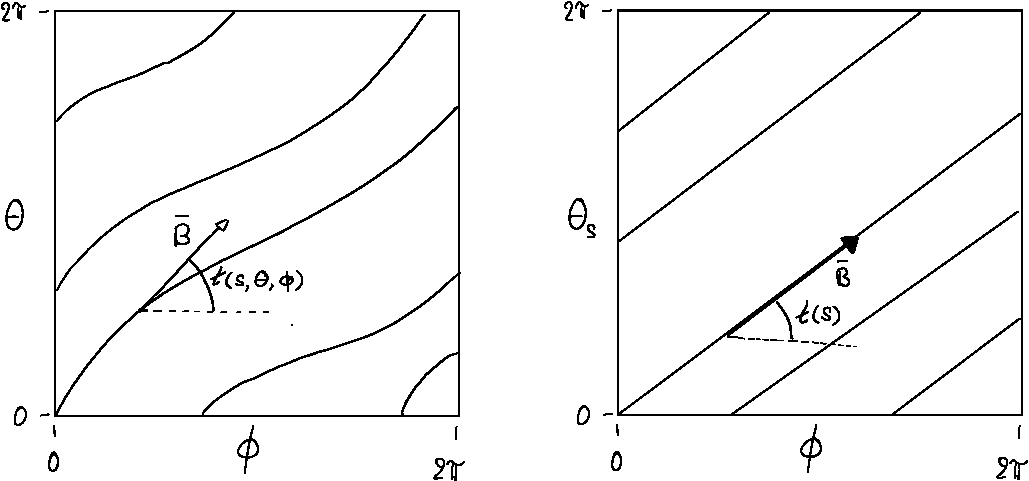
\includegraphics[width=\linewidth]{images/SketchFieldLine-crop.pdf}
	\caption{Sketch of three toroidal transits of a field line. Left: using general coordinates $(\theta,\zeta)$ and right: using straight field line coordinates $(\theta_s,\zeta)$.}
	\label{fig sketch field line}
\end{figure}

Equation (\ref{equation perp force balance}) implies that $\mathbf{B}\cdot\nabla p=0$, \textit{i.e.} the pressure is constant along a field line. If the pressure profile is smooth and not constant in any region, then equation (\ref{equation perp force balance}) implies that magnetic field lays on surfaces of constant pressure, thereby generating magnetic surfaces. Assuming the existence of rational magnetic surfaces where $\nabla p\neq 0$ is however the source of diverging currents, as we shall discuss in the sections (\ref{sec ideal mhd currents})-(\ref{sec. diverging currents}). 

The normalized pressure is defined as the ration between the plasma pressure and the magnetic pressure,
\begin{equation}
	\beta = \frac{2\mu_0 p}{B^2},
\end{equation}
with $B=|\mathbf{B}|$. Generally, the normalized pressure is either evaluated on the magnetic axis, with $\beta_0=2\mu_0 p_0/B_0^2$, where the subscript denotes an evaluation on the magnetic axis, or averaged other the plasma volume,
\begin{equation}
	\bar\beta = \frac{1}{\mathcal{V}_P} \iiint_{\mathcal{V}_P} \frac{2\mu_0 p}{B^2} dv,
\end{equation}
with $\mathcal{V}_P$ the plasma volume and $dv$ a volume element.

To finish this section, we define the flux surface average of a function $f(\psi,\theta,\zeta)$ as the volume average of $f$ between two neighboring magnetic surfaces \citep{helanderTheoryPlasmaConfinement2014}. The volume enclosed by a magnetic surface is
\begin{equation}
	V_{\psi_t} = \int_0^{\psi_t} d\psi \int_0^{2\pi} d\theta \int_0^{2\pi} \sqrt{g}d\zeta,
\end{equation}
with $\sqrt{g}$ the coordinate $(\psi_t, \theta, \zeta)$ jacobian. The flux surface average of $f$ is then
\begin{equation}
	\langle f \rangle = \frac{1}{V'(\psi_t)}\iint \frac{f dS}{|\nabla \psi_t|} = \left.\iint \frac{f dS}{|\nabla \psi_t|} \middle/ \iint\frac{dS}{|\nabla \psi_t|} \right.,
\end{equation}
with $dS=\sqrt{g}|\nabla\psi_t|d\theta d\zeta$. One important property of the flux surface average is that
\begin{equation}
	\langle \mathbf{B}\cdot\nabla f\rangle = 0. \label{eq.property_flux_average}
\end{equation}



\subsection{Ideal MHD solution in an axisymmetric cylinder}\label{appendix jxb=grad p solution}
As an illustration, we solve here the ideal MHD equilibrium equations (\ref{equation perp force balance})-(\ref{equation div B ideal mhd}) in an axisymmetric cylinder of length $L$ and radius $a$ (see Figure \ref{fig. cylinder sketch}). We work with cylindrical coordinate $(r,\theta,z)$. We assume that the cylinder boundary is a magnetic surface, \textit{i.e.} $\mathbf{B}\cdot\nabla r=0$ at $r=a$. Assuming symmetries along $\theta$ and $z$ (equivalent to axisymmetry in a toroidal geometry), we immediately from Eq.(\ref{equation perp force balance}) get that $p=p(r)$, \textit{i.e.} isopressure surfaces are cylinders with constant radii. Since the magnetic field lies on constant pressure surfaces, axisymmetry implies the existence of magnetic surfaces everywhere.

\begin{figure}
	\centering
	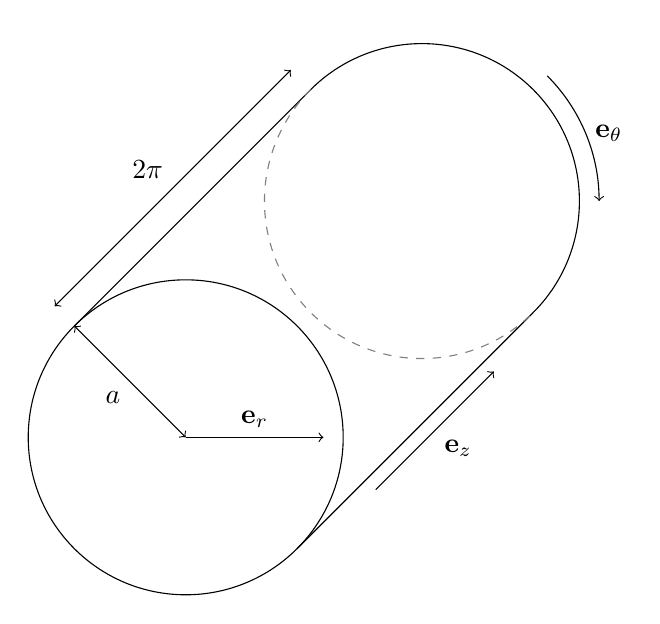
\begin{tikzpicture}
		\def\r{2}
		\def\L{3}
		\draw (0,0) circle (\r);
		\draw ({-\r*cos(45)},{\r*sin(45)}) -- ({-\r*cos(45)+\L},{\r*sin(45)+\L});
		\draw ({\r*cos(45)},{-\r*sin(45)}) -- ({\r*cos(45)+\L},{-\r*sin(45)+\L});
		\draw ({\r*cos(45)+\L},{-\r*sin(45)+\L}) arc (-45:135:\r);
		\draw[dashed,color=gray] ({-\r*cos(45)+\L},{\r*sin(45)+\L}) arc (135:315:\r);
		\draw[<-] ({\r+\L+0.25},{\L}) arc (0:45:{\r+0.25}) node[midway,anchor=west] {$\mathbf{e}_\theta$};
		\draw[->] (0,0) -- (\r-0.25,0) node[midway,above] {$\mathbf{e}_r$};
		\draw[->] ({\r*cos(45)+0.25+\L/4},{-\r*sin(45)+\L/4}) -- ({\r*cos(45)+3*\L/4+0.25},{-\r*sin(45)+3*\L/4}) node[midway,anchor=north west] {$\mathbf{e}_z$};
		\draw[<->] (0,0) -- ({-\r*cos(45)},{\r*sin(45)}) node[midway,anchor=north east] {$a$};
		\draw[<->] ({-\r*cos(45)-0.25},{\r*sin(45)+0.25})-- ({-\r*cos(45)+\L-0.25},{\r*sin(45)+\L+0.25}) node[midway,anchor=south east] {$2\pi$};
	\end{tikzpicture}
	\caption{Sketch of a plasma cylinder}
	\label{fig. cylinder sketch}
\end{figure}

We now search for a solution to the equilibrium equation. One gets from equation (\ref{equation div B ideal mhd})
\begin{align}
\frac{1}{r}\frac{\partial}{\partial r}(r B_r) &= 0, 
\end{align}
which, once the boundary condition is applied, leads to $B_r=0$. In addition, exploiting Ampere's law, we write the current densities as
\begin{align}
	\mu_0J_r &= 0\\
	\mu_0J_\theta &= -\frac{\partial B_z}{\partial r}\\
	\mu_0J_z &= \frac{1}{r}\frac{\partial}{\partial r}(rB_\theta).
\end{align} 
Finally, taking the cross product of the current density with the magnetic field and rearranging the terms, one gets
\begin{equation}
	\frac{d}{dr}\left(\mu_0p + \frac{B_\theta^2 + B_z^2}{2}\right) + \frac{B_\theta^2}{r} = 0.
\end{equation}

The equilibrium is thus completely determined if one provides (i) a pressure profile $p(r)$ and (ii) a constraint on either the poloidal or toroidal magnetic field --- for example by providing the poloidal flux profile $\psi_p(r)$, or the rotational transform profile $\iotabar(r)$.


% ================================================ CURRENTS ================================================
\subsection{Currents in ideal MHD equilibria}\label{sec ideal mhd currents}
The current density can be written as the sum of a component parallel to the magnetic field $J_\parallel \hat{\mathbf{b}}$, with $\hat{\mathbf{b}}=\mathbf{B}/B$ and of a component perpendicular to the magnetic field $\mathbf{J}_\perp$, required to counter-balance the pressure gradient in the force balance. Following \citet{helanderTheoryPlasmaConfinement2014}, we write the perpendicular current by taking the cross product of $\mathbf{B}$ with Eq.(\ref{equation perp force balance}),
\begin{equation}
	\mathbf{J}_\perp = \frac{\mathbf{B}\times\nabla p}{\mathbf{B}^2}.
\end{equation}
Parallel current $J_\parallel$ are then generated to ensure charge conservation (Eq.(\ref{equation charge conservation})). Imposing $\nabla \cdot (J_\parallel\mathbf{\hat{b}}) = - \nabla\cdot\mathbf{J}_\perp$ leads to 
\begin{equation}
	J_\parallel = u(\psi_t,\theta,\zeta)\frac{dp}{d\psi_t}B + \frac{\langle J_\parallel B\rangle B}{\langle B^2\rangle},
\end{equation}
where $(\psi_t,\theta,\zeta)$ are the toroidal flux, a poloidal angle and a toroidal angle, and $\langle\cdot\rangle$ denotes a flux surface average. Note that here we assume that magnetic surfaces exist, and that the toroidal flux is monotonously increasing from the plasma core to the plasma edge so that it can be used as a radial coordinate. The function $u(\psi_t,\theta,\zeta)$ satisfies
\begin{equation}
	\nabla\cdot\left(u\mathbf{B}p'+\frac{\mathbf{B}\times\nabla\psi_t}{B^2}p'\right) = 0.
\end{equation}
Using the vectorial identity $\nabla\cdot(f\mathbf{v})=v\cdot\nabla f+f\nabla\cdot\mathbf{v}$, with $f$ a scalar and $\mathbf{v}$ a vector, we get
\begin{equation}
	\nabla\cdot\left(u\mathbf{B}+\frac{\mathbf{B}\times\nabla\psi_t}{B^2}\right) = 0, \label{eq.div_eq_u}
\end{equation}
which can be casted as a magnetic differential equation for $u$, 
\begin{equation}
	\mathbf{B}\cdot\nabla u = -(\mathbf{B}\times\nabla\psi_t)\cdot\nabla\left(\frac{1}{B^2}\right). \label{eq.diff_u}
\end{equation}
The total current density is thus
\begin{equation}
	\mathbf{J} = \frac{\mathbf{B}\times\nabla p}{\mathbf{B}^2} + \left(u(\psi_t,\theta,\zeta)\frac{dp}{d\psi_t} + \frac{\langle J_\parallel B\rangle}{\langle B^2\rangle}\right)\mathbf{B}, \label{equation current density}
\end{equation}
where the first term on the right hand side of Eq.(\ref{equation current density}) is the \emph{diamagnetic current}, the second is the \emph{Pfirsch-Schl\"uter current} and the last term encompasses other parallel currents, such as the externally driven currents (Ohmic, \ac{ECCD}, \ac{NBCD}) or bootstrap current (see section \ref{sec.bootstrap}).

We now discuss the relative importance of the different terms in Eq.(\ref{equation current density}) in setting the net toroidal current in a stellarator. To do so, we work in Boozer coordinates (see appendix \ref{appendix  boozer coordinates}) and we take the flux surface average of the total current density projected in the Boozer toroidal direction, $\mathbf{J}\cdot\nabla\zeta_b$ {\color{red} source from A. Alonso}.

We start by looking at the contribution from the diamagnetic current density. We write the magnetic field in its contravariant form,
\begin{equation}
	\mathbf{B} = I(\psi_t)\nabla\theta_b + G(\psi_t)\nabla\zeta_b + K(\psi_t,\theta_b,\zeta_b)\nabla\psi_t, 
\end{equation}
with $I(\psi_t)$ the net toroidal current enclosed inside a magnetic surface, $G(\psi_t)$ the net poloidal current outside a magnetic surface, and $K(\psi_t,\theta_b,\zeta_b)$ a function. The diamagnetic current flux surface average is then
\begin{align}
	\langle\mathbf{J}_\perp\cdot\nabla\zeta_b\rangle &= p'\left\langle \left(\frac{\mathbf{B}\times\nabla\psi_t}{B^2}\right)\cdot\nabla\zeta_b\right\rangle\\
	&= p'\left\langle \frac{1}{\sqrt{g}B^2}(I(\psi_t) \mathbf{e}_{\zeta_b} - G(\psi_t)\mathbf{e}_{\theta_b})\cdot\nabla\zeta_b\right\rangle = pI(\psi_t)\left\langle \frac{1}{B^2 \sqrt{g_b}} \right\rangle,
\end{align} 
where we used the relation $\mathbf{e}_{\theta_b} = \sqrt{g_b}\nabla\theta_b\times\nabla\psi_t$ and $\mathbf{e}_{\zeta_b} = \sqrt{g_b}\nabla\psi_t\times\nabla\theta_b$, with $\mathbf{e}_{\theta_b},\mathbf{e}_{\zeta_b}$ the covariant basis vector of the Boozer coordinates $\theta_b$ and $\zeta_b$ respectively. Using the expression of the jacobian in Boozer coordinates (Eq.\ref{eq.jacobian_boozer}), we get
\begin{equation}
	\langle\mathbf{J}_\perp\cdot\nabla\zeta_b\rangle = \frac{Ip'}{G+\iotabar I}.
\end{equation}
Interestingly, the diamagnetic current contributes to the net toroidal current only if there are other sources of toroidal current in the plasma.

To evaluate the contribution from the Pfirsch-Schl\"uter current density, we write the magnetic field using its covariant representation (Eq.(\ref{eq.covariant_b_boozer})), which implies
\begin{equation}
	\mathbf{B}\cdot\nabla\zeta_b = (\nabla\psi_t\times\nabla\theta_b + \iotabar \nabla\zeta_b\times\nabla\psi_t)\cdot\nabla\zeta_b = \frac{1}{\sqrt{g_b}}. \label{eq.B_dot_nabla_phi}
\end{equation}
We thus obtain
\begin{equation}
	\left\langle u\mathbf{B}\cdot\nabla\zeta_b p'\right\rangle = p' \left\langle \frac{u}{\sqrt {g_b}}\right\rangle = \frac{p'}{G+\iotabar I}\langle uB^2 \rangle.
\end{equation}
From Eq.(\ref{eq.div_eq_u}), we can write
\begin{equation}
	uB^2 = \mathbf{B}\cdot\left(u\mathbf{B}+\frac{\mathbf{B}\times\nabla\psi_t}{B^2}\right) = \mathbf{B}\cdot\nabla f,
\end{equation}
where we leveraged the relation $\nabla\cdot\nabla f = 0$. Finally, using the property $\langle \mathbf{B}\cdot\nabla f\rangle = 0$ (Eq.(\ref{eq.property_flux_average})), we obtain that the flux averaged Pfirsch-Schl\"uter current density is
\begin{equation}
	\langle  u\mathbf{B}\cdot\nabla\zeta_b p'\rangle = 0.
\end{equation}

Externally driven currents and the bootstrap current provide a final contribution of 
\begin{equation}
	\frac{\langle J_\parallel B\rangle}{\langle B^2\rangle}\langle \mathbf{B}\cdot\nabla\zeta_b\rangle =  \frac{\langle J_\parallel B\rangle}{\langle B^2\rangle} \left\langle\frac{1}{\sqrt{g_b}}\right\rangle = \frac{\langle J_\parallel B\rangle}{G + \iotabar I},
\end{equation}
where we used Eq.(\ref{eq.B_dot_nabla_phi}) and the expression of the boozer coordinate jacobian, Eq.(\ref{eq.jacobian_boozer}). The flux surface average of the total current density projected on $\nabla\zeta_b$ is then
\begin{equation}
	\langle \mathbf{J}\cdot\nabla\zeta_b\rangle =  \frac{Ip'}{G+\iotabar I} + \frac{\langle J_\parallel B\rangle}{G + \iotabar I}. \label{eq.flux_av_current_mhd}
\end{equation}
We are now in position to estimate which current contributes the most to the net toroidal current. Taking the ration of the first and second terms on the right hand side of Eq.(\ref{eq.flux_av_current_mhd}), we find
\begin{align}
	\frac{I p'}{\langle J_\parallel B\rangle} \sim \frac{I p }{J_{\parallel,\phi} B \psi_{t}} \sim \frac{I}{I_{\parallel,\phi}} \frac{p}{B^2} \sim \frac{I}{2I_{\parallel,\phi}}  \beta \sim \beta.
\end{align}
Here we assumed that $p'\sim p/\psi_t$, with $\psi_t=\pi a^2 B$, and $a$ the minor radius. As the magnetic field is mostly toroidal, $J_{\parallel}\sim J_{\parallel,\phi}$, and the net toroidal current generated by the $J_\parallel$ current density is $I_{\parallel,\phi}\sim J_{\parallel} \pi a^2$. As $\beta\ll 1$, we conclude that the main contribution to the flux averaged current density comes from the externally driven and bootstrap currents. The Pfirsch-Schl\"uter flux averaged current density vanishes, and the diamagnetic flux surface averaged current density is negligible. While the diamagnetic current is by construction included in any magnetic equilibrium calculation, it is thus crucial to include the contribution from the externally driven and bootstrap current to compute the full effect of the currents on the magnetic field.




% ================================================ CLASSES OF EQUILIBRIA ================================================
\subsection{Classes of well posed 3D magnetic equilibria}\label{sec. diverging currents}

As we shall see, the magnetic differential equation (\ref{eq.diff_u}) has important implications on the existence of 3D magnetic equilibria with nested magnetic surfaces. In the discussion below, we follow \citet{helanderTheoryPlasmaConfinement2014} and solve equation (\ref{eq.diff_u}) assuming the existence of magnetic surfaces and using the coordinate system $(\psi_t,\theta_b,\zeta_b)$, where $(\theta_b,\zeta_b)$ are the poloidal and toroidal Boozer angles (see appendix \ref{appendix boozer coordinates}). We write the functions $u(\psi_t,\theta_b,\zeta_b)$ and $B^{-2}(\psi_t,\theta_b,\zeta_b)$ as double Fourier series,
\begin{align}
	u(\psi_t,\theta_b,\zeta_b) &= \sum_{m,n} u_{mn}(\psi_t) e^{i(m\theta_b-n\zeta_b)}\label{eq.u_fourier_expansion}\\
	\frac{1}{B^2}(\psi_t,\theta_b,\zeta_b) &= \sum_{m,n} h_{mn}(\psi_t) e^{i(m\theta_b-n\zeta_b)}\label{eq.b_fourier_expansion},
\end{align}
and we express the magnetic field $\mathbf{B}$ on the contravariant Boozer coordinate basis,
\begin{equation}
	\mathbf{B} = I(\psi_t)\nabla\theta_b + G(\psi_t)\nabla\zeta_b + K(\psi_t,\theta_b,\zeta_b)\nabla\psi_t.\label{eq.b_contravariant_boozer}
\end{equation}
Substituting Eq.(\ref{eq.b_contravariant_boozer}) in Eq.(\ref{eq.diff_u}), we can write the left hand side as
\begin{align}
	\mathbf{B}\cdot\nabla u &= \mathbf{B}\cdot\nabla\theta_b\frac{\partial u}{\partial \theta_b} + \mathbf{B}\cdot\nabla\zeta_b\frac{\partial u}{\partial \zeta_b} + \mathbf{B}\cdot\nabla\psi_t\frac{\partial u}{\partial \psi_t} \\
	&= \left(\iotabar \frac{\partial u}{\partial \theta_b} + \frac{\partial u}{\partial \zeta_b}\right)\mathbf{B}\cdot\nabla\zeta_b,
\end{align}
and the right hand side as
\begin{align}
	\left(\mathbf{B}\times\nabla\psi_t\right)\cdot\nabla \frac{1}{B^2} &= \left(I\nabla\theta_b\times\nabla\psi_t + G\nabla\zeta_b\times\nabla\psi_t\right)\cdot\nabla\frac{1}{B^2}\\
	&= \frac{1}{\sqrt{g}}\left(G\frac{\partial}{\partial\theta_b} - I \frac{\partial}{\partial \zeta_b}\right)\frac{1}{B^2},
\end{align}
with $\nabla\psi_t\cdot(\nabla\theta_b\times\nabla\zeta_b) = 1/\sqrt{g}$ the inverse of the Boozer coordinate jacobian. Substituting the Fourier series (\ref{eq.u_fourier_expansion})-(\ref{eq.b_fourier_expansion}) for $u$ and $1/B^2$, we finally obtain
\begin{equation}
	(m\iotabar - n)u_{mn} = (mG + nI)h_{mn},
\end{equation}
where we used the property of Boozer coordinates $\sqrt{g_b}^{-1}=\mathbf{B}\cdot\nabla\zeta_b$. Rearranging the terms, we get an expression for $u_{mn}$,
\begin{equation}
	u_{mn} = \frac{(mG + nI)}{m\iotabar - n}h_{mn} + \Delta_{mn}\delta(\psi_t-\psi_{t,mn}),\label{eq.umn}
\end{equation}
where $\Delta_{mn}$ is a constant and $\psi_{t,mn}$ is the toroidal flux enclosed by the rational magnetic surface where $\iotabar=n/m$. The Pfirsch-Schl\"uter current density, Eq.(\ref{equation current density}), has then two parts; one is a delta function, and the other is
\begin{equation}
	J_{mn} = \frac{(mG + nI)}{m\iotabar - n}h_{mn}p'(\psi_t).\label{diverging current}
\end{equation}

At rational surfaces, where $\iotabar=n/m$, the current density (\ref{diverging current}) diverges as a $1/x$ singularity if the pressure gradient is finite and if the magnetic field harmonics $h_{mn}$ is non zero. This particular singularity might be nonphysical since the integrated net toroidal current could diverge; note that the current density $\Delta_{mn} p'(\psi_t) \delta(\psi_t-\psi_{t,mn})$, is on the other hand well defined, since it is a finite quantity once integrated. To circumvent the issue of nonphysical diverging currents and obtain well defined, ideal MHD solutions, one has to consider constrained classes of equilibria.

One possibility is to consider equilibria where the inverse magnetic field squared resonant harmonic is zero at each rational surface, \emph{i.e.} $h_{mn}=0$, discussed by \citet{Weitzner2014}. Another is to relax the assumption of smooth, continuous solutions, and consider rotational transform profiles that are stepped --- essentially jumping from irrational to irrational values, and entirely avoiding rational surfaces. This has been discussed by \citet{Loizu2015a}. Similarly, one could consider equilibria where the pressure is constant around resonant surfaces. Since rationals are dense in $\mathbb{R}$, the pressure profile is either stepped or fractal. Stepped pressure equilibria have been proven to exist close to axisymmetry by \citet{Bruno1996}. A combination of the second and third class discussed above, where the rotational transform profile and the pressure profile are alternatively constant, can be constructed to obtain solution with continuous profiles \citep{Hudson2017a}. Recently, a final class of equilibria has been proposed by Y-H. Huang {\color{red} add source}, where the delta function current densities in Eq.(\ref{eq.umn}) would modify the radial dependency of $G$, $I$, $p$ and $\iotabar$ such that the current density $J_{mn}$ does not diverge at rational surfaces.

In the remaining of this thesis, we will work with stepped-pressure equilibria. The reason is three-fold: (i) these equilibria are numerically tractable, \textit{e.g.} there are no fractal structure in the considered profiles, (ii) solutions with magnetic islands and chaos can be obtained and (iii) solutions have been proven to exist under some conditions. In particular, we will work with \ac{MRxMHD} equilibria, which are a specific class of stepped-pressure equilibria and can be seen as a combination of Taylor states, described in the following section.



\section{Taylor state}
\label{section taylor state}
One trivial way to solve the ideal MHD equation (\ref{equation perp force balance})-(\ref{equation div B ideal mhd}) is to consider the case where the pressure is flat, \textit{i.e.} $\nabla p=0$ everywhere. Therefore the diverging current density, equation (\ref{diverging current}), is zero. The force balance equation (\ref{equation perp force balance}) implies that $\mathbf{J}\times\mathbf{B}=0$, meaning that the current density is parallel to the magnetic field, $\mathbf{J}=\mu(r,\theta,\zeta)\mathbf{B}$.

The Taylor state \citep{Taylor1974,Taylor1986} is a particular case of force-free fields where the function $\mu$ is a constant, which give the Taylor equilibrium equation,
\begin{equation}
	\nabla\times\mathbf{B}=\mu\mathbf{B}. \label{equation Taylor state}
\end{equation}

Solution to the equation (\ref{equation Taylor state}) in a slab and a cylinder are derived below.

\subsection{Solution in a plasma slab}
We solve equation (\ref{equation Taylor state}) in a plasma Slab. We use Cartesian coordinates $(x,y,z)$ with $(\mathbf{e}_x,\mathbf{e}_y,\mathbf{e}_z)$ the basis vector. The plasma slab is bounded by two surfaces at $x=0$ and $x=a$, and we assume that these surfaces are magnetic surfaces, \textit{i.e.} $\mathbf{B}\cdot\mathbf{e}_x=0$. We assume periodic boundary conditions in the $y$ and $z$ directions, and that the equilibrium is axisymmetric, \textit{i.e.} $\mathbf{B}=\mathbf{B}(x)$ (see Figure \ref{fig. plasma slab}).

\begin{figure}
	\centering
	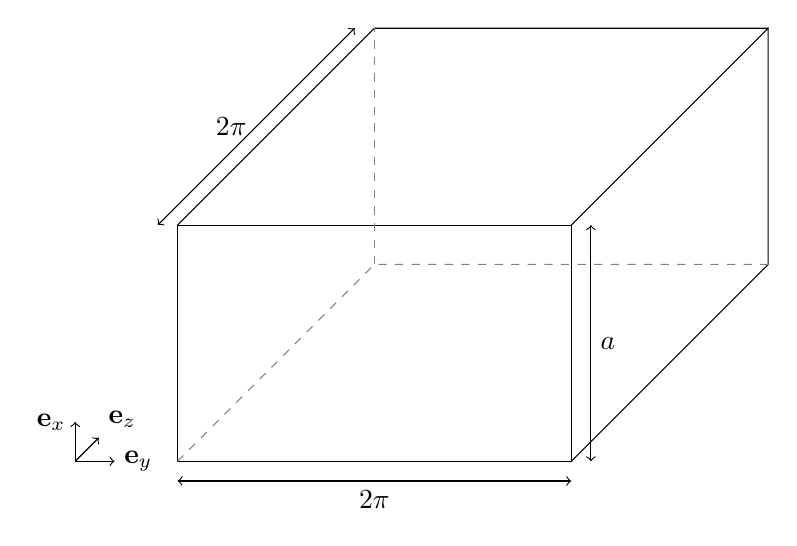
\begin{tikzpicture}
		\def\x{5}
		\def\a{3}
		\draw (0,0) -- (\x,0) -- (\x,\a) -- (0,\a) -- cycle;
		\draw (\x,0) -- ({\x*1.5},{\x*0.5}) --  ({\x*1.5},{\a+\x*0.5}) -- (\x,\a);
		\draw ({\x*1.5},{\a+\x*0.5}) -- ({\x*0.5},{\a+\x*0.5}) -- (0,\a);
		\draw[dashed, color=gray] (0,0) -- ({\x*0.5},{\x*0.5}) --  ({\x*1.5},{\x*0.5});
		\draw[dashed, color=gray] ({\x*0.5},{\x*0.5}) --  ({\x*0.5},{\a+\x*0.5});
		\draw[->] (-1.3,0) -- (-1.3,0.5) node[anchor=east] {$\mathbf{e}_x$};
		\draw[->] (-1.3,0) -- (-0.8,0) node[anchor=west] {$\mathbf{e}_y$};
		\draw[->] (-1.3,0) -- (-1.0,0.3) node[anchor=south west] {$\mathbf{e}_z$};
		\draw[<->] (0,-0.25) -- (\x,-0.25) node[midway,below] {$2\pi$};
		\draw[<->] (-0.25,\a) -- ({\x*0.5-0.25},{\a+0.5*\x}) node[midway,left] {$2\pi$};
		\draw[<->] ({\x+0.25},0) -- ({\x+0.25},\a) node[midway,right] {$a$};
	\end{tikzpicture}
	\caption{Sketch of a plasma slab}
	\label{fig. plasma slab}
\end{figure}

The equation $\nabla\cdot\mathbf{B}=0$ implies that $B_x=0$, while equation (\ref{equation Taylor state}) can be written as
\begin{align}
	\frac{\partial B_z}{\partial x} &= -\mu B_y\\
	\frac{\partial B_y}{\partial x} &= \mu B_z,
\end{align}
whose solution is
\begin{align}
	B_y &= B_0 \cos(\mu (x + x_0))\\
	B_z &= -B_0 \sin(\mu (x + x_0)),
\end{align}
where $B_0$ and $x_0$ are integration constant, which can be fixed by providing, for example, a constraint on the poloidal and toroidal fluxes. Note that, in this geometry, three constants (or constraints) $(\mu,B_0,x_0)$ have to be provided to fully determine the equilibrium.

\subsection{Solution in a plasma cylinder}
We now solve equation (\ref{equation Taylor state}) in a plasma cylinder. We use cylindrical coordinates $(r,\theta,z)$, and assume that the $z$ coordinate is $2\pi$-periodic. The plasma cylinder is bounded by a single surface at $r=a$, which we assume to be a magnetic surface,  \textit{i.e.} $\mathbf{B}\cdot\nabla r=0$ at $r=a$. Again, we assume the equilibrium to be axisymmetric, \textit{i.e.} $\mathbf{B}=\mathbf{B}(r)$ (see Figure \ref{fig. cylinder sketch}).

The equation $\nabla\cdot\mathbf{B}=0$ implies that $B_r=0$, and equation (\ref{equation Taylor state}) leads to
\begin{align}
	\mu B_\theta &= -\frac{\partial B_z}{\partial r}\\
	\mu B_z &= \frac{1}{r}\frac{\partial}{\partial r}(rB_\theta).
\end{align}
Defining $x=\mu r$, we thus obtain
\begin{equation}
	x^2 \frac{\partial^2 B_\theta}{\partial x^2} + x \frac{\partial B_\theta}{\partial x} + (x^2-1) B_\theta = 0,
\end{equation}
which we identify to Bessel's differential equation. The solutions are then
\begin{align}
	B_\theta &= B_0 J_1(\mu r)\\
	B_z &= B_0 J_0(\mu r),
\end{align}
where $J_i$ is the Bessel function of the $i^{\text{th}}$ order, and $B_0$ is an integration constant, which can be fixed by providing an additional constraint, for example the toroidal flux. Note that in a cylinder only two constants (or constraints) $(\mu,B_0)$ have to be provided to fully determine the equilibrium. This is in opposition to the plasma slab case, where three constants had to be provided. This difference is intransically linked to the topology of the domain; in a slab, there are two boundaries to the plasma, one at $x=0$ and one at $x=a$, while in a cylinder there is only one boundary, at $r=a$. 

These important topological properties are also true in toroidal geometries; two constants are required to fully determine the Taylor state in a torus, while three constants are required in a toroidal annulus.

\section{MRxMHD}
\label{section mrxmhd}
%The \ac{MRxMHD} theory \citep{Dewar2015, Hole2006} has been developed to address this question. \ac{MRxMHD} minimizes the \ac{MHD} energy functional \citep{kruskal_equilibrium_1958} while keeping the magnetic helicity and the magnetic fluxes constant \citep{Dewar2015} in a finite set of $N_{vol}$ nested volumes $\mathcal{V}_l$ at constant pressure (see Figure \ref{fig:Illustration_SPEC}) but otherwise allowing arbitrary, non-ideal variations in the magnetic field. Interfaces $\delta\mathcal{V}_l$ separating the volumes are ideal flux surfaces which therefore cannot undergo magnetic re-connection, effectively constraining discretely the magnetic field topology. In the limit of a single volume, $N_{vol}=1$, Taylor states \citep{Taylor1974, Taylor1986} are recovered, while in the limit of an infinite number of volumes, $N_{vol}\rightarrow\infty$, it has been proven that \ac{MRxMHD} recovers ideal \ac{MHD} (section \ref{section ideal mhd}) \citep{Dennis2013} in the limit of continuously nested flux surfaces, thereby bridging the gap between both theories.

Taylor states can not describe plasma equilibria with pressure profile. An alternative is proposed by the MRxMHD equilibrium model, which describes solutions to equations (\ref{equation perp force balance})-(\ref{equation div B ideal mhd}) assuming stepped-pressure profiles. The pressure steps are supported by magnetic surfaces $\mathcal{I}_l$, $l\in\{1,\ldots,N_{vol}\}$, with irrational rotational transform, \textit{i.e.} $\iotabar\in\mathbb{R}\setminus\mathbb{Q}$, which defines a finite number of volumes $\mathbf{V}_l$ between each pair of interface (see Figure \ref{fig:Illustration_SPEC}). In each volume, the magnetic field is described by a Taylor state, 
\begin{equation}
	\nabla\times\mathbf{B}=\mu_l\mathbf{B}. \label{eq.BeltramiEquation}
\end{equation}
We remark that while ideal \ac{MHD} equilibria are defined by two free functions (\textit{e.g.} the pressure and the rotational transform profiles, $p(\psi_t)$ and $\iotabar(\psi_t)$, or the pressure and the current profiles, $p(\psi_t)$ and $I_\zeta(\psi_t)$), \ac{MRxMHD} requires two scalars to determine the solution in a volume $\mathcal{V}_l$, in addition to the pressure and toroidal flux. This can be considered as three independent discrete profiles that are required to determine an equilibrium. Examples are $\{p_l, \mu_l, \psi_{p,l}\}_{l=1,\ldots,N_{vol}}$, $\{p_l, \mu_l, K_l\}_{l=1,\ldots,N_{vol}}$, with $K_l$ the magnetic helicity in volume $\mathcal{V}_l$, or $\{p_l,\iotabar^-_l,\iotabar^+_l\}_{l=1,\ldots,N_{vol}}$, with $\iotabar^\pm_l$ the rotational transform on the inner and outer side of the interface $\mathcal{I}_l$, as functions of $\{\psi_{t,l}\}_{l=1,\ldots,N_{vol}}$. The innermost volume is a special case, since it only has one boundary; the magnetic field in the innermost volume is thus fully determined by two scalars, for example $(\mu_1,\psi_{t,1})$.

The geometry of the volumes' boundary is chosen such that force balance is achieved, \textit{i.e.} the total pressure (plasma and magnetic pressure) is continuous across each volume interface $\mathcal{I}_l$,
\begin{equation}
	\left[\left[p + \frac{B^2}{2\mu_0}\right]\right]_l = 0, \label{eq.force_balance}
\end{equation}
where $[[x]]_l\equiv x_{l+1}-x_l$ denotes the discontinuity across interface $l^{\text{th}}$. The MRxMHD equilibrium can then be seen as a collection of nested Taylor state at equilibrium with one another. 

\begin{figure}
	\centering
	\begin{tikzpicture}
		\node[] (fig) at (0,0)
		{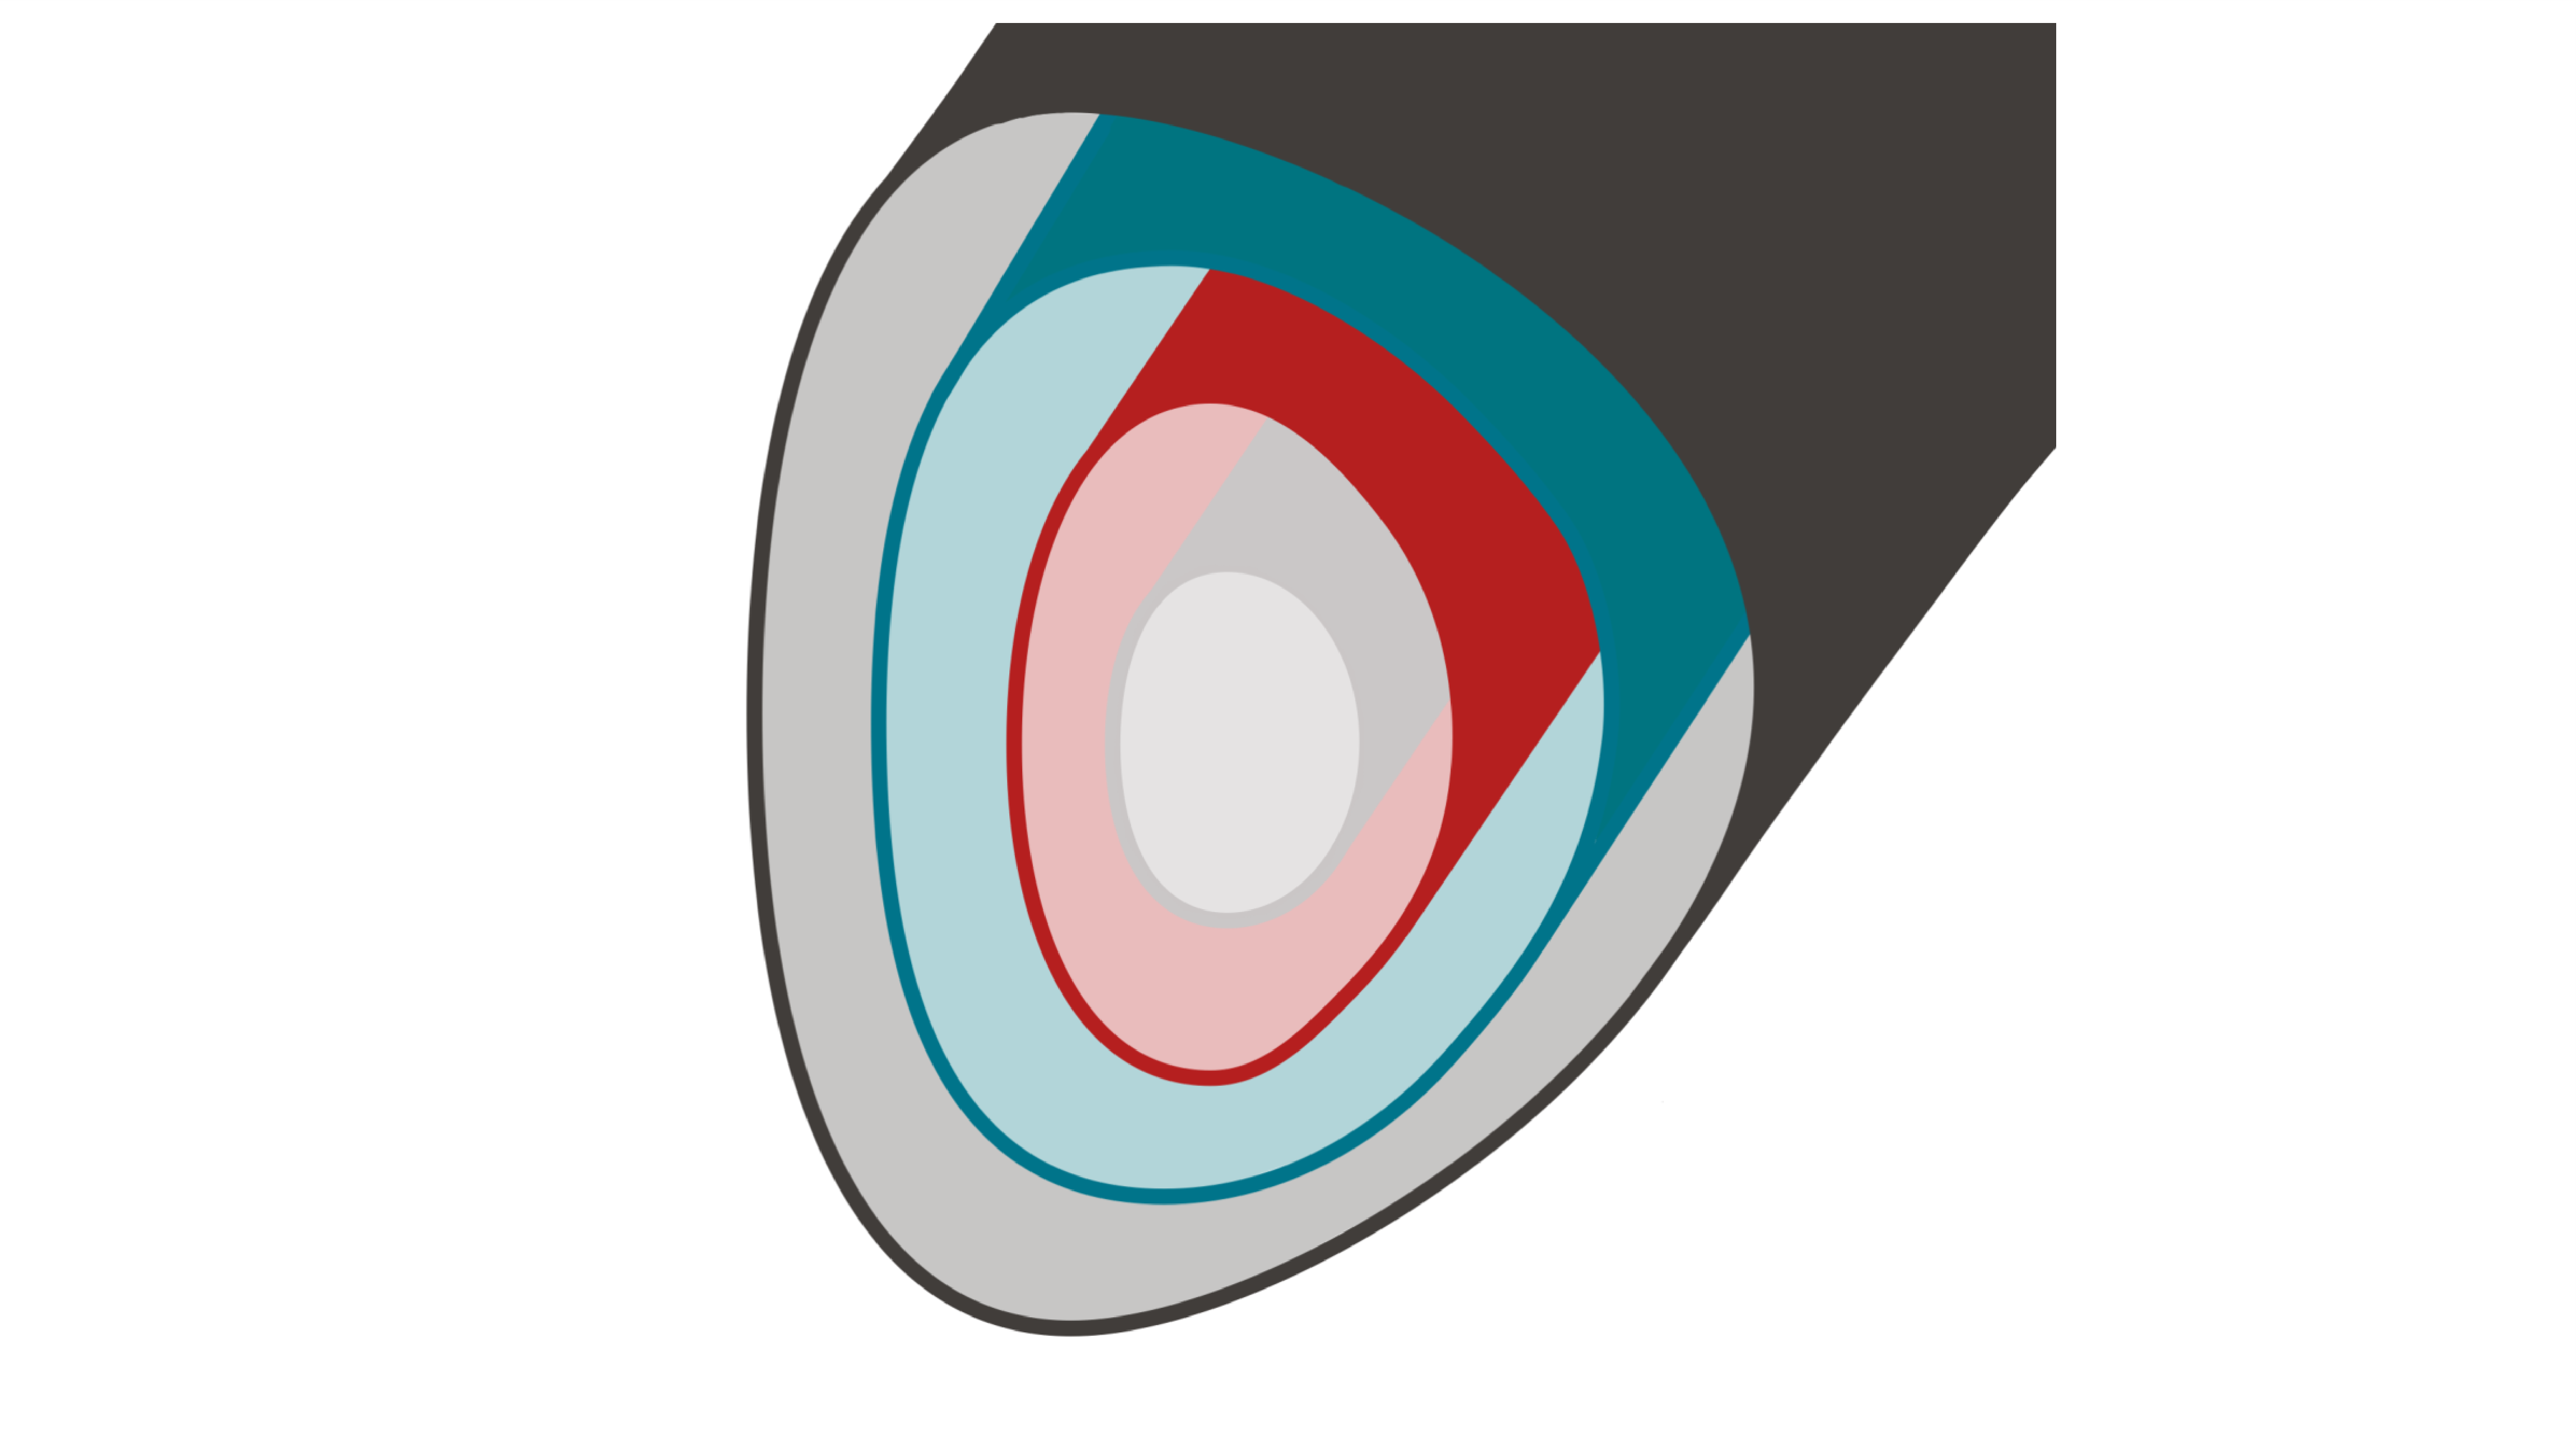
\includegraphics[width=0.9\textwidth]{main/Figures_CurrentConstraint/ABaillod_fig1.pdf}};
		%\draw (-5,-5) grid[] (5,5);
		\draw (-0.3 ,-0.3 ) node {$\mathcal{V}_1$};
		\draw (-1 ,-1 ) node {$\mathcal{V}_2$};
		\draw (-1.5 ,-1.5) node {$\mathcal{V}_3$};
		\draw (-2 ,-2.1 ) node {$\mathcal{V}_4$};
		\draw ( 0.0 , 1.0 ) node {$\mathcal{I}_1$};
		\draw ( 0.5 , 1.5 ) node {\color{white}$\mathcal{I}_2$};
		\draw ( 0.85 , 1.85 ) node {\color{white}$\mathcal{I}_3$};
		\draw ( 1.5 , 2.5 ) node {\color{white}$\mathcal{I}_4$};
	\end{tikzpicture}
	\caption{Illustration of 4 nested volumes, $\mathcal{V}_1$ to $\mathcal{V}_4$, separated by 4 interfaces, $\mathcal{I}_1$ to $\mathcal{I}_4$.}
	\label{fig:Illustration_SPEC}
\end{figure}

The MRxMHD class of equilibrium thus extends the Taylor state to equilibria with pressure gradients. Magnetic field line topologies are discretely constrained to be magnetic surfaces at the volumes' boundaries, while magnetic islands and magnetic field line chaos can be present in the volumes between the interfaces. Diverging currents, as described in section \ref{sec. diverging currents}, are avoided since pressure gradients are only supported by irrational magnetic surfaces. There are however some drawbacks; the magnetic field, and so the rotational transform, pressure and other physical profiles, are in general discontinuous across the interfaces. Finally, interfaces may not always exist --- either a magnetic island or magnetic field line chaos is present, or the pressure jump is too large for a single surface to support it \citep{Qu2021}. Therefore, care must be taken when constructing MRxMHD equilibria, and in their analysis. 


%In each volume $\mathcal{V}_l$, the solution to Eq.(\ref{eq.BeltramiEquation}) is completely determined by three scalars (for example $\{\mu_l,\psi_{t,l},\psi_{p,l}\}$), the geometry of interfaces bounding the volume and a boundary condition for the magnetic field normal to the interfaces $\mathbf{B}_l\cdot\hat{\mathbf{n}}_k$, $k=\{l-1,l\}$, with $\hat{\mathbf{n}}_k$ a unit vector perpendicular to the interface $k$. In \ac{MRxMHD}, the interfaces are imposed to be flux surfaces, with $\mathbf{B}_l\cdot\hat{\mathbf{n}}_k=0$. In the innermost volume, which is topologically different from the others, only two scalars are required in addition to the geometrical degrees of freedom and the condition $\mathbf{B}_1\cdot\hat{\mathbf{n}}_1=0$.


\subsection{Currents in MRxMHD}\label{ch2.mrxmhd_currents}


\textit{Disclaimer: this section is heavily based on the publication by \citet{Baillod2021}.}

One important part of the work presented in this thesis is the implementation of a new capability in the SPEC code (introduced in chapter \ref{ch3.SPEC}) to run at fixed net toroidal current profile. The numerical implementation will be explained in great details in section \ref{sec. current constraint}; we describe in this section how currents are represented in the MRxMHD theory.

In \ac{MRxMHD}, two spatially distinct net toroidal current profiles co-exist, namely currents flowing in the volumes, $\{I^v_{l,\zeta}\}_{l=\{1,\ldots,N_{vol}\}}$, and surface currents flowing at the volumes' interfaces, $\{I^s_{l,\zeta}\}_{l=\{1,\ldots,N_{vol}-1\}}$ (current sheets), where the subscript $\zeta$ refers to the toroidal angle. The volume current $I^v_{l,\zeta}$ in volume $\mathcal{V}_l$ is easily evaluated using Eq.(\ref{eq.BeltramiEquation}) and Ampere's law,
\begin{equation}
    \mu_0I^v_{l,\zeta} = \mu_l\iint_{\mathcal{S}_{l,\zeta}} \mathbf{B}\cdot\mathbf{dS}_{l,\zeta} = \mu_l \psi_{t,l},
    \label{eq.volume_current}
\end{equation}
where $\mathcal{S}_{l,\zeta}$ is a constant-$\zeta$ surface in volume $\mathcal{V}_l$ and $\mathbf{dS}_{l,\zeta}$ is the differential surface element normal to $\mathcal{S}_{l,\zeta}$. Volume currents include externally driven currents such as \ac{ECCD}, \ac{NBCD} or Ohmic current. Eq.(\ref{eq.volume_current}) might be surprising since toroidal currents are usually expressed in terms of functions of the poloidal fluxes and not the toroidal fluxes. In essence, the poloidal flux dependence is contained in $\mu_l$, which is related to the parallel current density, as $\mu_l = \mu_0 \mathbf{j}_l\cdot\mathbf{B}_l / B_l^2$, with $\mathbf{j}_l$ the current density in volume $\mathcal{V}_l$. The surface current $I^s_{l,\zeta}$ at interface $\mathcal{I}_l$ can be evaluated using Ampere's law
\begin{equation}
    \mu_0I^s_{l,\zeta} = \int_{\Gamma _l} \left[\left[ \mathbf{B} \right]\right]_l \cdot \mathbf{dl} = \oint_0^{2\pi} \left[\left[B_\theta\right]\right] d\theta \equiv 2\pi \left[\left[ \tilde{B}_{\theta} \right]\right]_l, \label{eq.surf_current}
\end{equation}
where $\Gamma_l$ is a closed curve following the interface $\mathcal{I}_l$ poloidally and $\tilde{B}_{\theta}$ is the $m=n=0$ Fourier mode of the covariant component of the poloidal magnetic field. In Eq.(\ref{eq.surf_current}), the poloidal and toroidal angles, $\theta$ and $\zeta$, are as-of-yet arbitrary. However the surface currents $I^s_{l,\zeta}$ are, as expected, independent of these angles choice, since the surface currents only depend on the $m=n=0$ mode of the field. Surface currents represent all equilibrium pressure-driven currents, such as diamagnetic, Pfirsch-Schl\"uter, and bootstrap currents, as well as shielding currents arising when an ideal interface is positioned on a resonance \citep{Loizu2015}.


\subsubsection{Currents discretization}
Typically, continuous current profiles are provided by analytical models or after equilibrium reconstruction using experimental data. We now discuss how these profiles can be represented in the framework of \ac{MRxMHD}. Consider an externally driven current profile, \textit{e.g} \ac{ECCD}, provided as the enclosed toroidal current as a function of the toroidal magnetic flux, \textit{i.e.} $I_{\zeta,ECCD}(\psi_t)$, and a pressure-driven current profile, \textit{e.g.} the bootstrap current, provided similarly as the enclosed toroidal current as a function of the toroidal flux, $I_{\zeta,BS}(\psi_t)$. We also assume that the pressure profile, $p(\psi_t)$, the number of volumes, $N_{vol}$, and their enclosed toroidal fluxes, $\{\psi_{t,l}\}_{l=1,\ldots,N_{vol}}$, are given (see Figure \ref{fig:sketch_pressure}). The question of how many volumes and where to position their interfaces to best represent a given pressure profile is not addressed in this chapter.

\begin{figure}
    \centering
    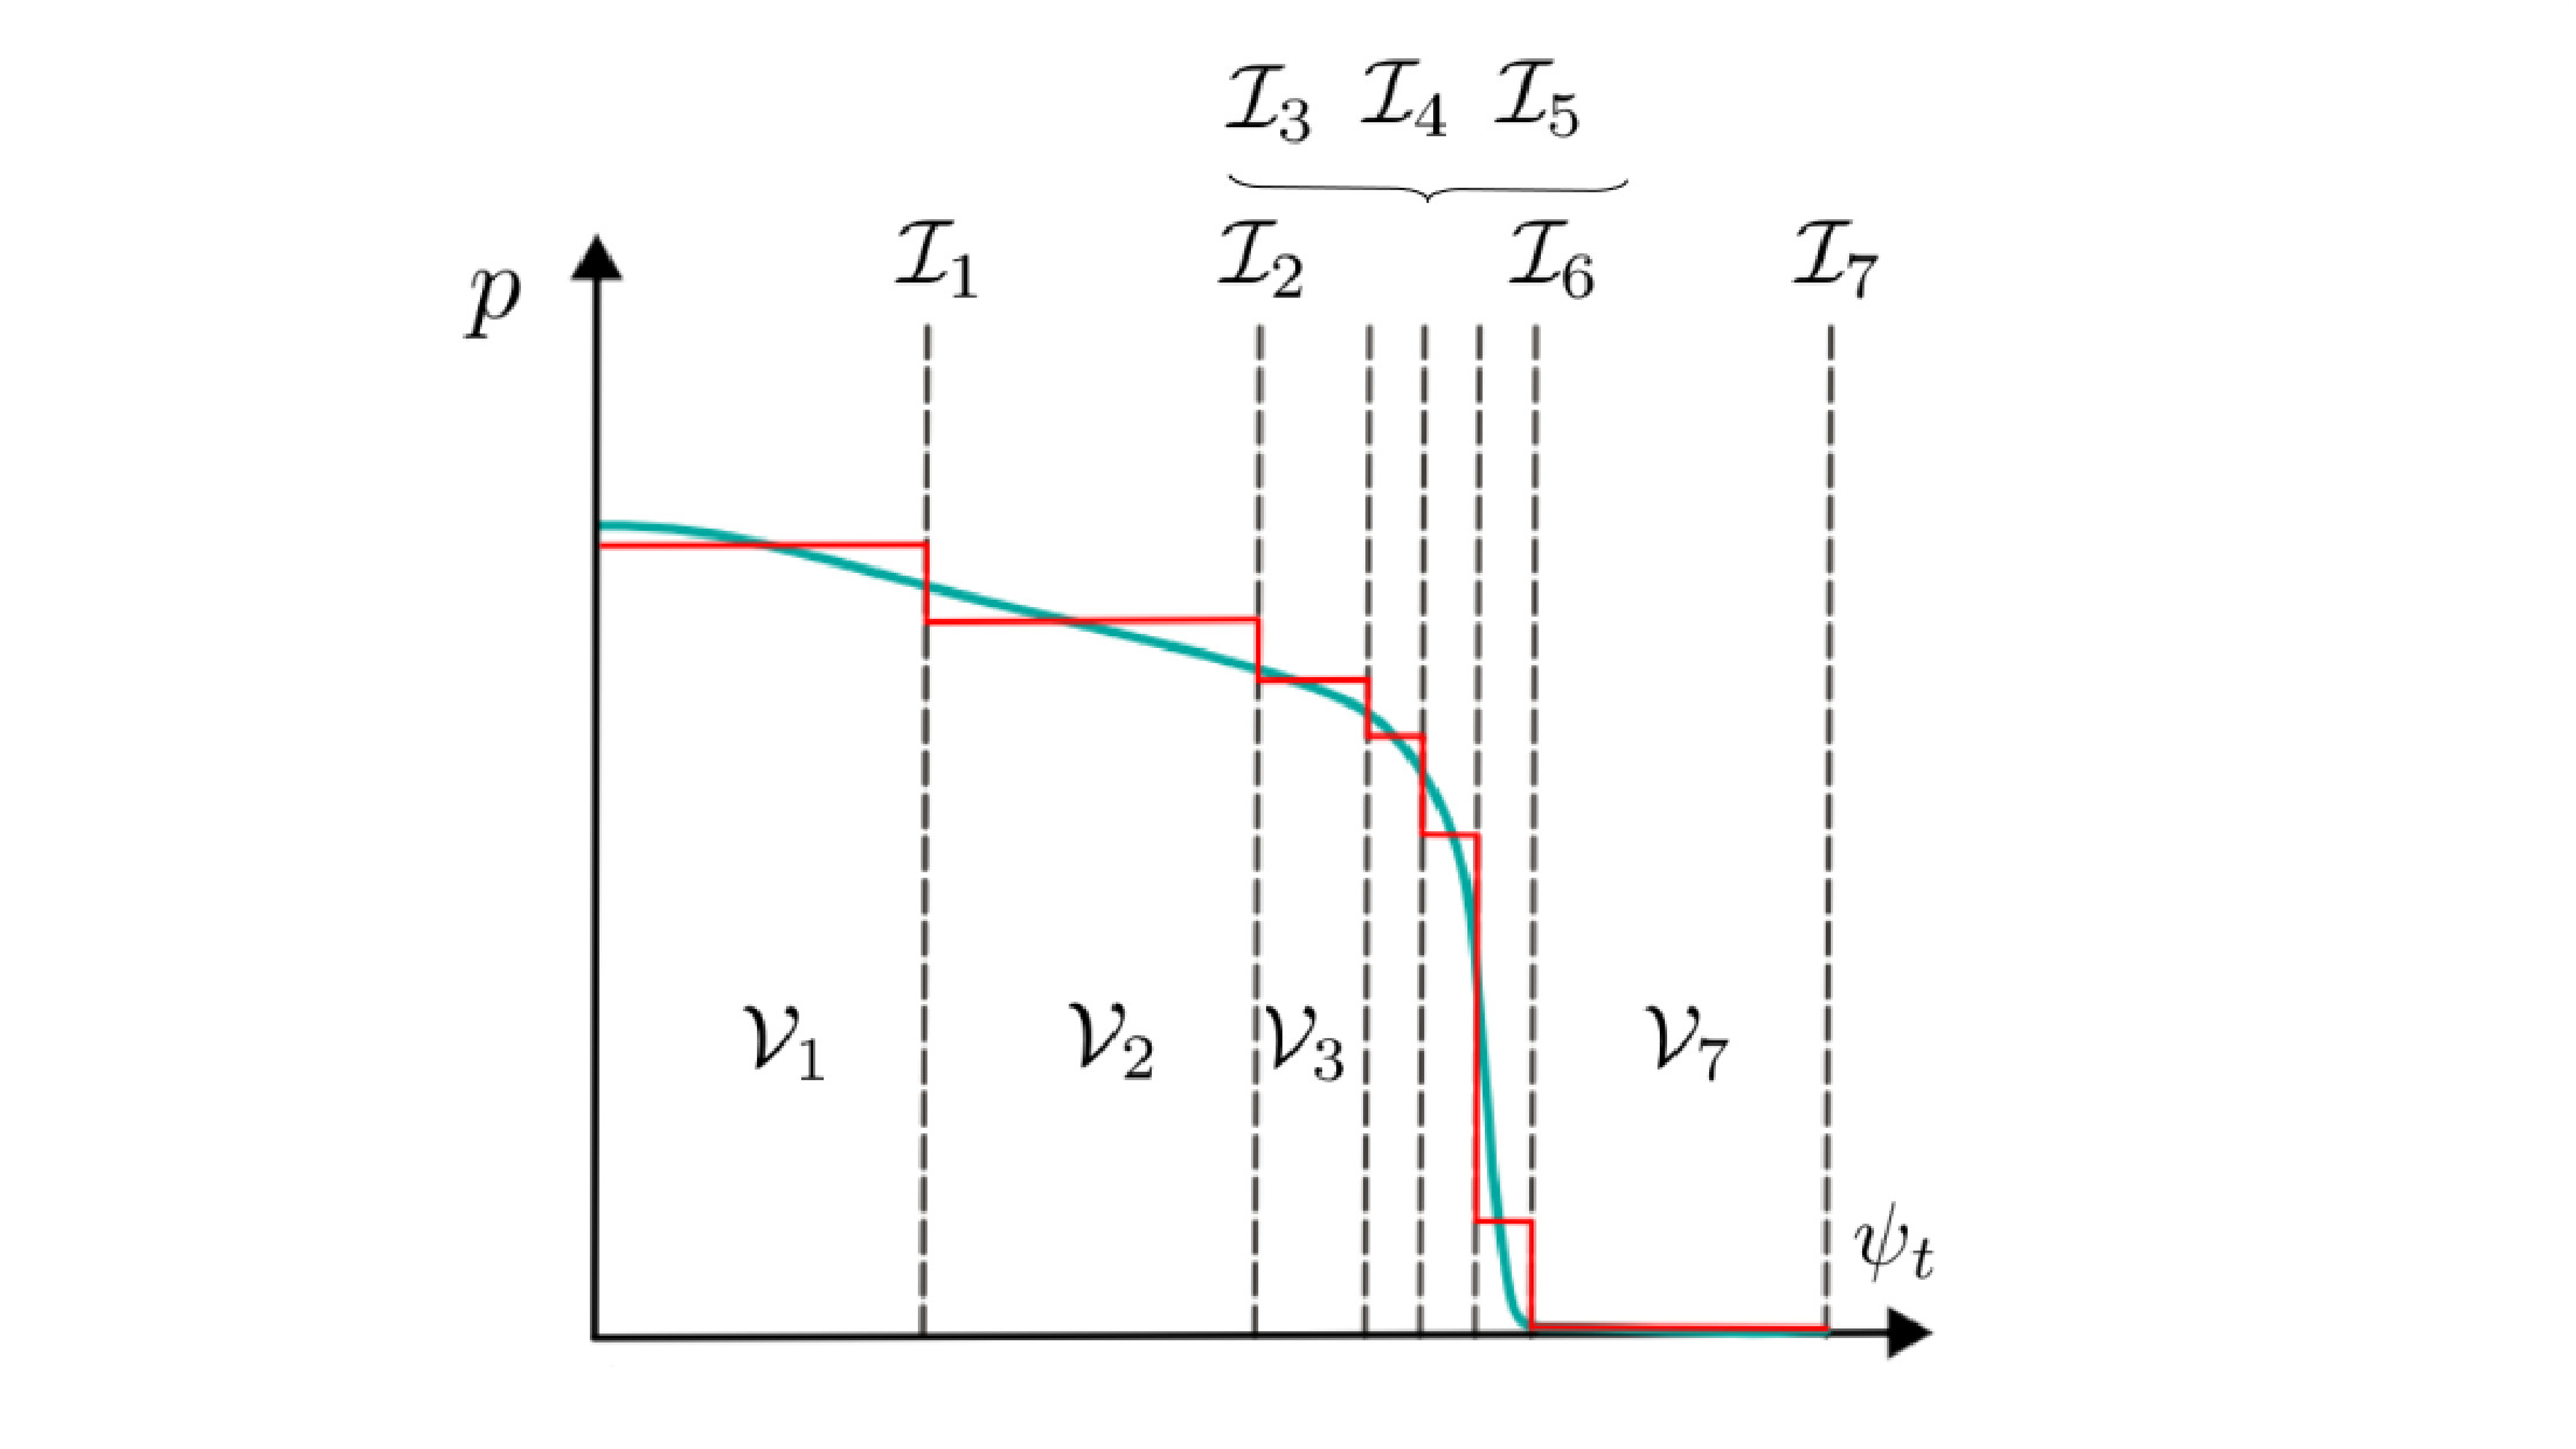
\includegraphics[width=\linewidth]{main/Figures_CurrentConstraint/ABaillod_fig2.pdf}
    \caption{Sketch of a pressure profile as a function of the toroidal flux. Blue: continuous pressure profile obtained via experiment or analytical model. Red: SPEC discretized pressure profile. Black dashed lines: volume interfaces.}
    \label{fig:sketch_pressure}
\end{figure}

A proposed representation of these current density profiles in \ac{MRxMHD} is achieved as follows. The \ac{ECCD} current is an externally driven, parallel current and is thus represented as a volume current since it flows parallel to the field lines; on the other hand, the bootstrap current is a pressure-driven, self-generated current and is represented as a surface current, since it is localized at the pressure gradients. Volume currents are obtained by integrating the externally driven current density in each volume (Figure \ref{fig:sketch_eccd}), which is simply given by the difference

\begin{figure}
    \centering
    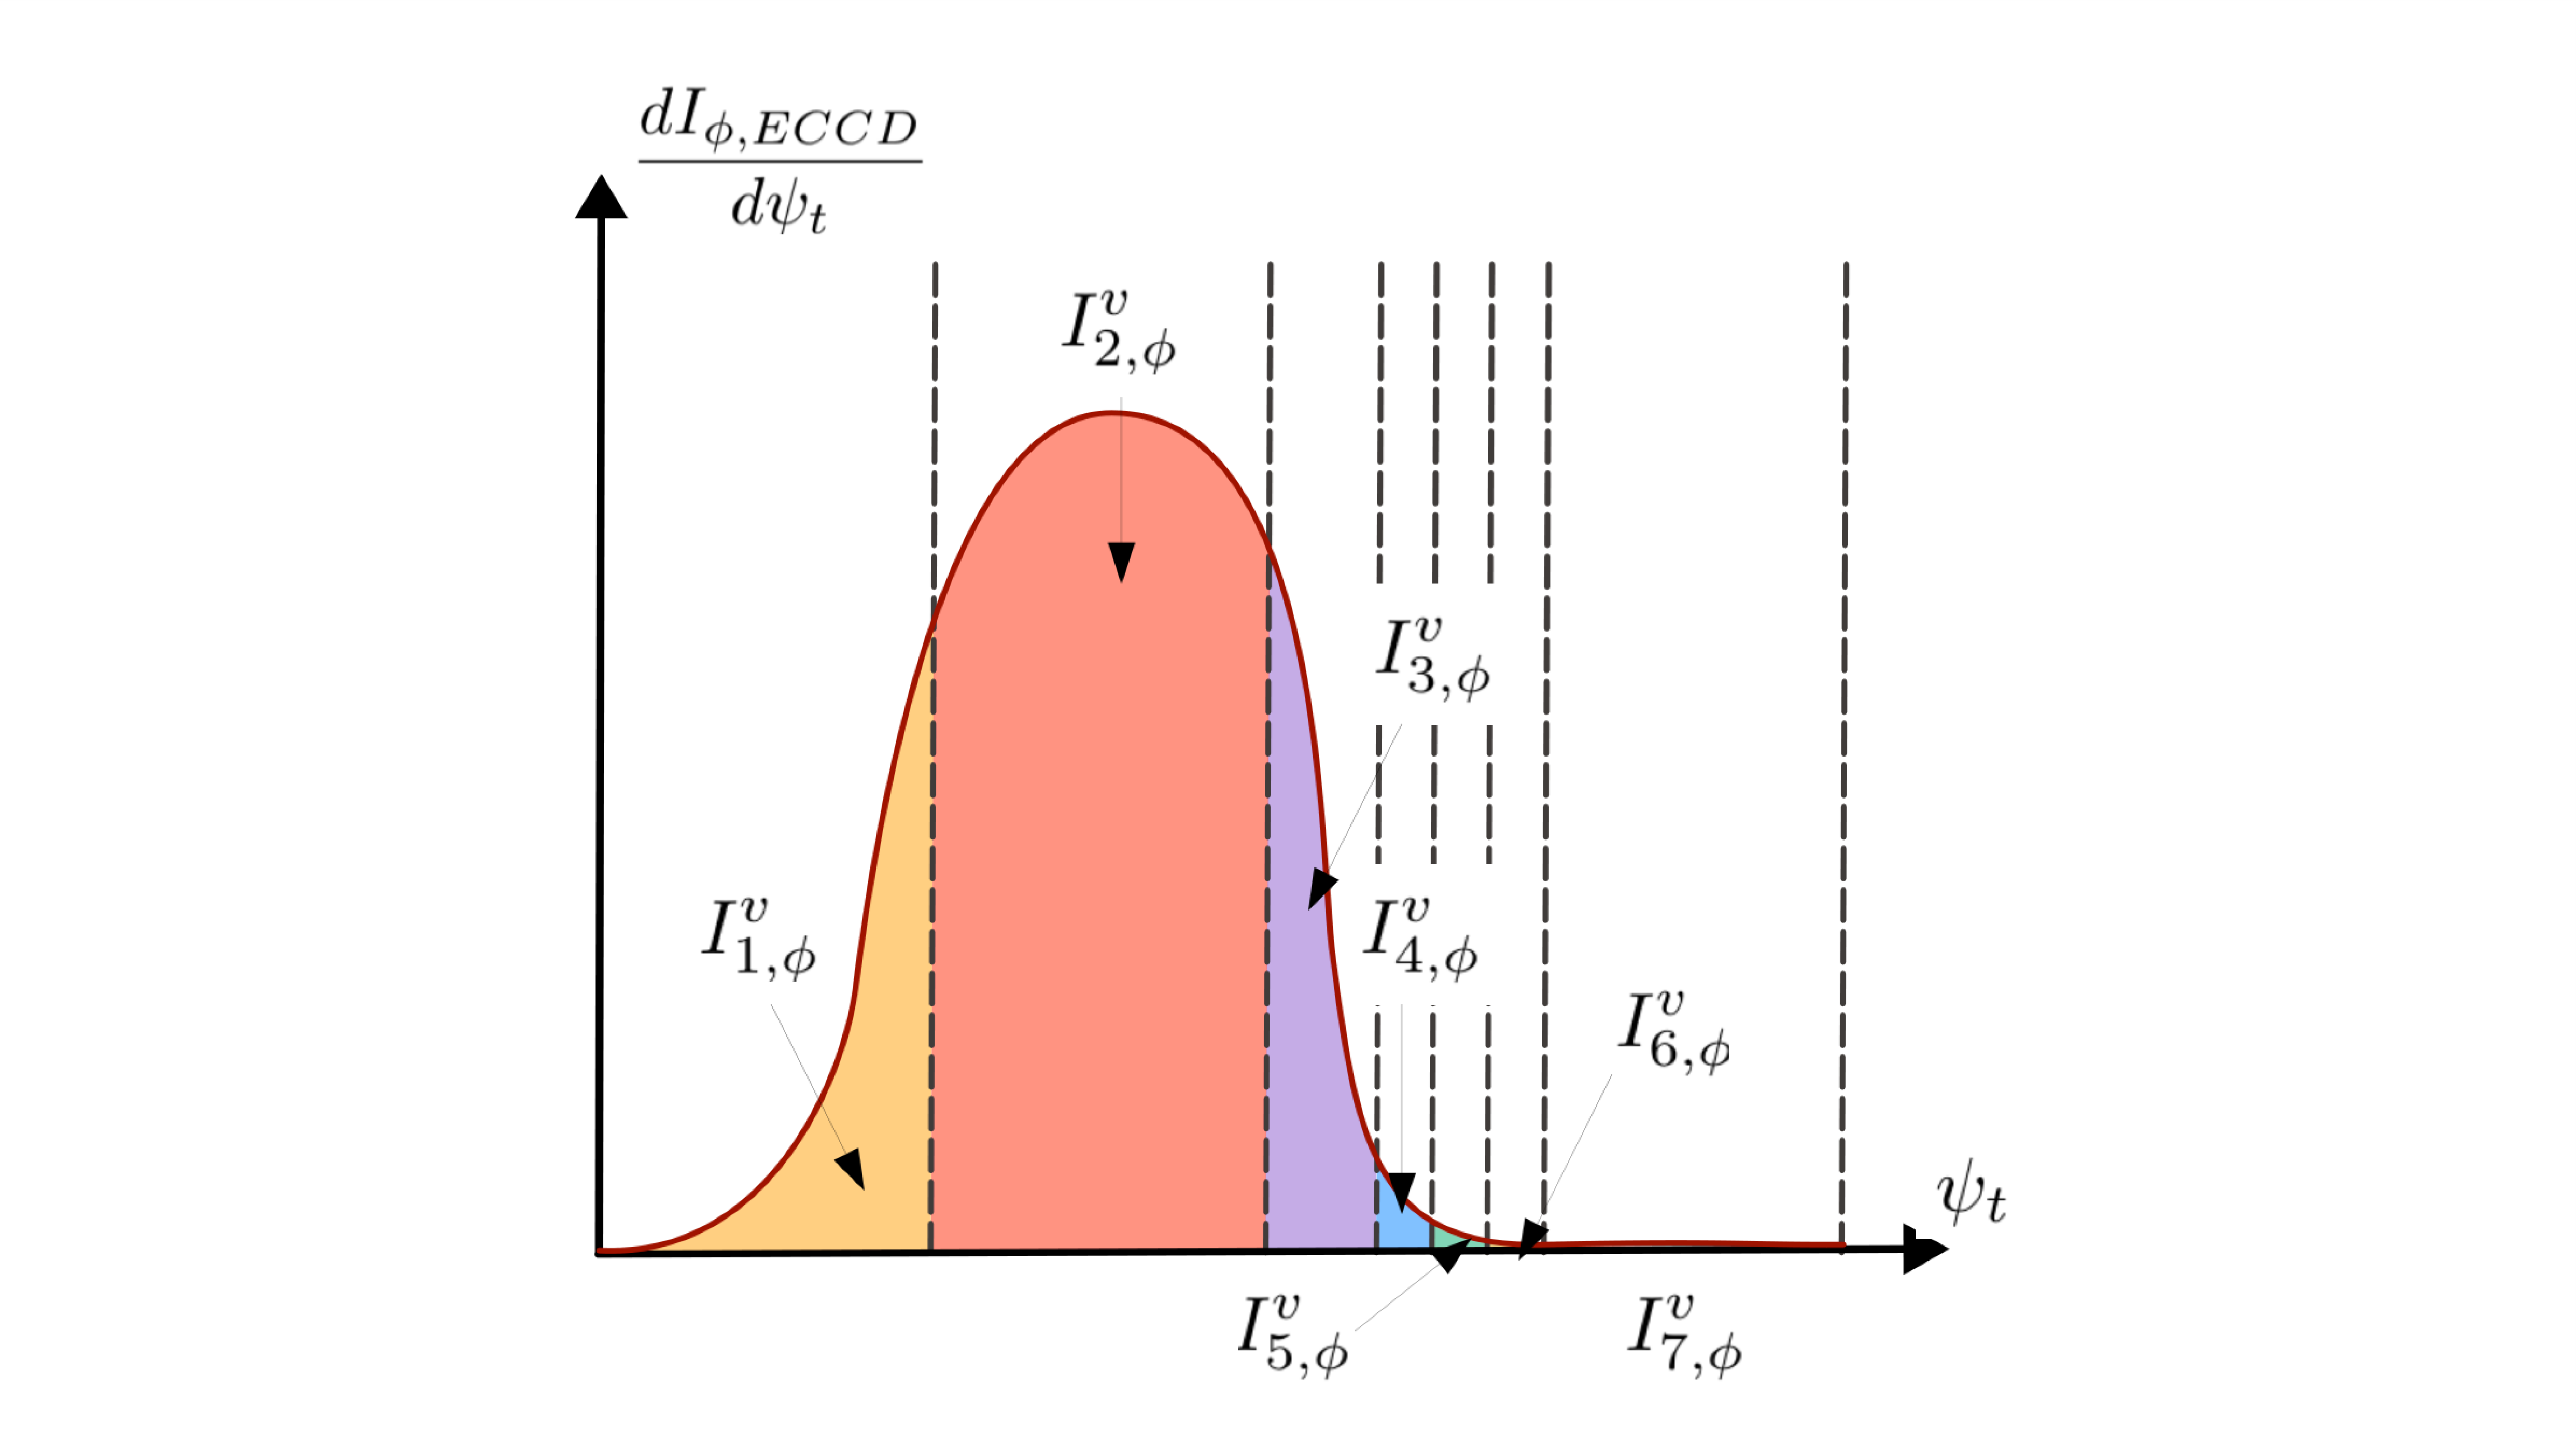
\includegraphics[width=\linewidth]{main/Figures_CurrentConstraint/ABaillod_fig3.pdf}
    \caption{Sketch of externally driven current density (red curve). Colored area correspond to the \ac{MRxMHD} volume current. Black dashed lines represent volume interfaces.}
    \label{fig:sketch_eccd}
\end{figure}


\begin{equation}
    I^v_{l,\zeta} = I_{\zeta,ECCD}(\psi_{t,l}) - I_{\zeta,ECCD}(\psi_{t,l-1}), \label{eq.rep_volume_current}
\end{equation}
and the surface currents are obtained by integrating the pressure driven current density around each interface (Figure \ref{fig:sketch_bootstrap}), which is expressed as

\begin{equation}
    I^s_{l,\zeta} = I_{\zeta,BS}(\psi_{l,out}) - I_{\zeta,BS}(\psi_{l,in}), \label{eq.rep_surface_current}
\end{equation}
with

\begin{align}
    \psi_{l,in} &= \begin{cases}
    0 & \text{if } l=1\\
    \frac{\psi_{t,l-1} + \psi_{t,l}}{2} & \text{otherwise}
    \end{cases}\label{eq.surf_disc1} \\
    \psi_{l,out} &= \begin{cases}
    \psi_{a} & \text{if } l=N_{vol}-1\\
    \frac{\psi_{t,l} + \psi_{t,l+1}}{2} & \text{otherwise}
    \end{cases},\label{eq.surf_disc2}
\end{align}
with $\psi_{a}$ the total toroidal magnetic flux enclosed by the plasma. In Eqs.(\ref{eq.surf_disc1})-(\ref{eq.surf_disc2}), care has been taken for the first and last interfaces, where the surface of integration has been extended to include the current density from the magnetic axis and up to the plasma boundary. Note that this difference in the definition of the first and last surface currents vanishes as the number of volumes $N_{vol}$ is increased. Eqs.(\ref{eq.rep_volume_current})-(\ref{eq.surf_disc2}) are only one possible discretization of the continuous current profiles, proposed by the authors for illustration. Advantages of this particular representation are (1) that the total toroidal current is always preserved and (2) that the currents are approximately localized at the same location in the discretized than in the continuous case.


\begin{figure}
    \centering
    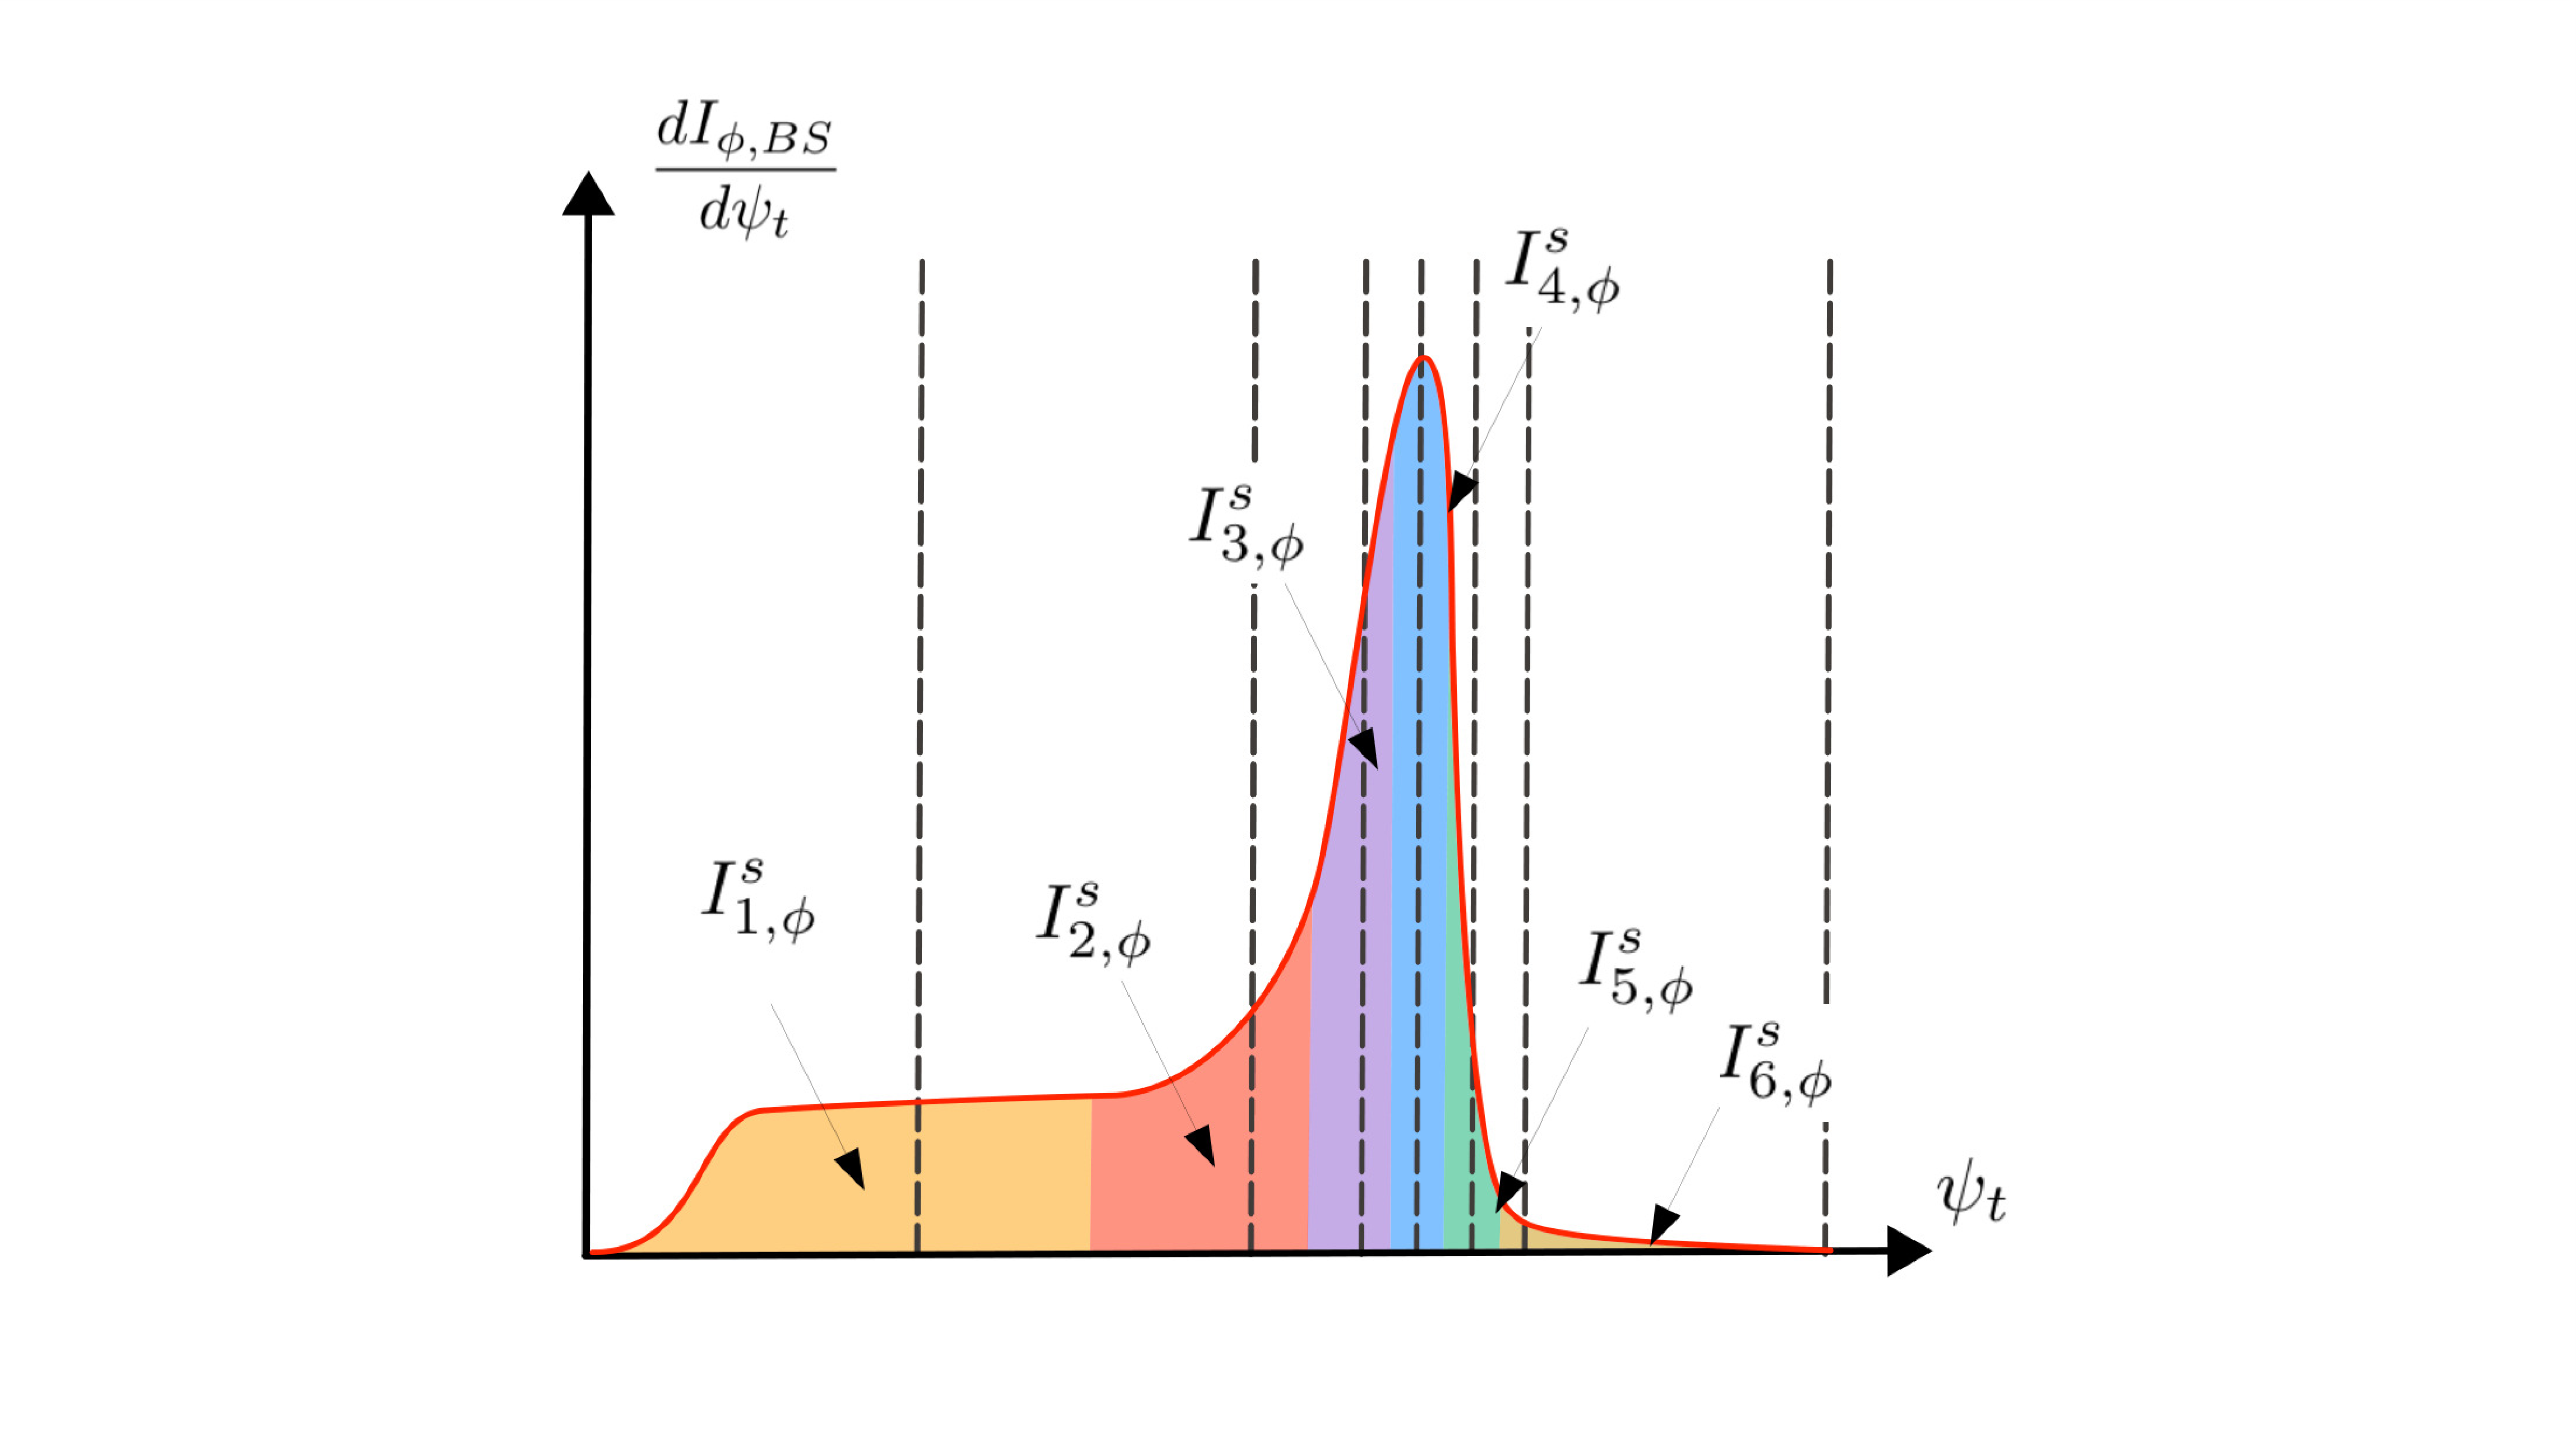
\includegraphics[width=\linewidth]{main/Figures_CurrentConstraint/ABaillod_fig4.pdf}
    \caption{Sketch of pressure driven current density. Colored area correspond to the \ac{MRxMHD} surface current. Black dashed lines represent volume interfaces.}
    \label{fig:sketch_bootstrap}
\end{figure}







\section{Energy principles}
To complete this chapter, we show here that the ideal MHD equilibrium equations, the Taylor state, and the MRxMHD equations can all be derived from an energy principle. In fact, all three models derive from the same energy functional, which is minimized under different topological constraints. We first start by discussing the relation between magnetic helicity and field line topology conservation.

% ================================================ HELICITY ================================================
\subsection{Conservation of field line topology}
%In ideal \ac{MHD}, it is assumed that the plasma is \emph{ideal}, meaning that it has zero resistivity. There are thus no mechanisms for energy dissipation and the plasma is not allowed to reconnect, \textit{i.e.} only plasma displacements that conserve the topology of magnetic field lines are allowed. It has been shown \citep{woltjer_theorem_1958} that this constraint is equivalent to conserving the magnetic helicity $K$ in any plasma volume $\mathcal{V}_i$, with
An important property of the ideal MHD model is that the magnetic helicity $K$ is conserved everywhere under ideal MHD evolution, with
\begin{equation}
	K = \iiint_{\mathcal{V}_i} d\mathbf{x}^3 \mathbf{A} \cdot \mathbf{B},
\end{equation}
where $\mathbf{A}=\nabla\times\mathbf{B}$ is the magnetic vector potential. Indeed, we find
\begin{align}
	\frac{dK}{dt} &= \iiint_{\mathcal{V}_i} d\mathbf{x}^3 \frac{d\mathbf{A}}{dt}\cdot\mathbf{B} + \mathbf{A}\cdot\frac{d\mathbf{B}}{dt} + \iint_{\delta\mathcal{V}_i} \mathbf{A}\cdot\mathbf{B}(\mathbf{n}\cdot\mathbf{v})d\mathbf{x}^2, \\
	&= -2\iiint_{\mathcal{V}_i}\mathbf{E}\cdot\mathbf{B} d\mathbf{x}^3 + \iint_{\delta\mathcal{V}_i}(\mathbf{n}\times\mathbf{A})\cdot(\mathbf{E}+\mathbf{v}\times\mathbf{B})d\mathbf{x}^2,
\end{align}
where $\mathcal{V}_i$ is any volume in the plasma bounded by magnetic surfaces, $\mathbf{n}$ is a unit vector normal to $\delta \mathcal{V}_i$, and $\mathbf{v}$ is the velocity describing the motion of the boundary $\delta\mathcal{V}_i$. Applying the ideal Ohm's law (Eq.(\ref{ideal Ohms law})), we obtain $dK/dt = 0$, \textit{i.e.} the magnetic helicity is conserved everywhere in the plasma according to ideal MHD. Indeed, the magnetic helicity has been shown to be approximately conserved during fast reconnection events \citep{bergerIntroductionMagneticHelicity1999}, and has been observed to be conserved in tokamak sawtooth crashes \citep{Heidbrink2000}. 

Magnetic helicity can be linked to the magnetic field line topologies. One can show \citep{moffattDegreeKnottednessTangled1969, arnoldTopologicalPropertiesMagnetic1998, bergerIntroductionMagneticHelicity1999} that the magnetic helicity is the sum of the Gauss linking number over every pair of field lines within a volume, where the Gauss linking number is a measure of how intertwined field lines are (see Figure \ref{fig gauss linking number}). Note the following implication: in ideal MHD, the magnetic helicity is conserved \emph{everywhere}, meaning that the magnetic topology is conserved during plasma motion. Therefore, no magnetic reconnection event can be discribed by ideal MHD dynamics.

\begin{figure}
	\hspace{.125\linewidth}
	\subfloat[][Gauss linking number is 1]{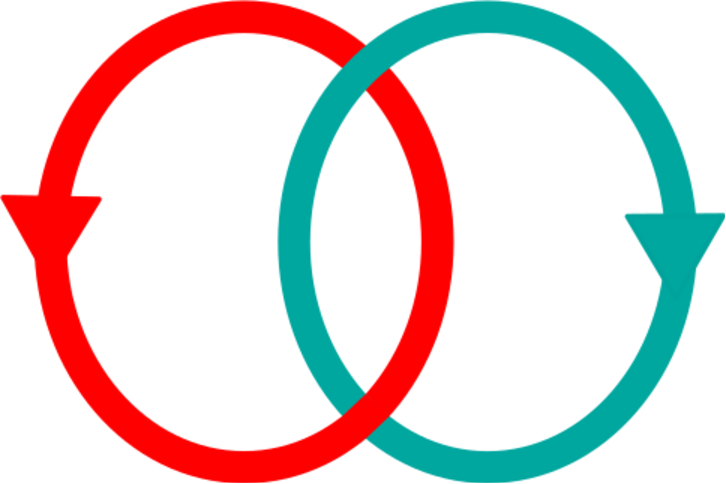
\includegraphics[height=4cm]{images/Gauss_linking_number_001.pdf}}
	\hfill
	\subfloat[][Gauss linking number is 3]{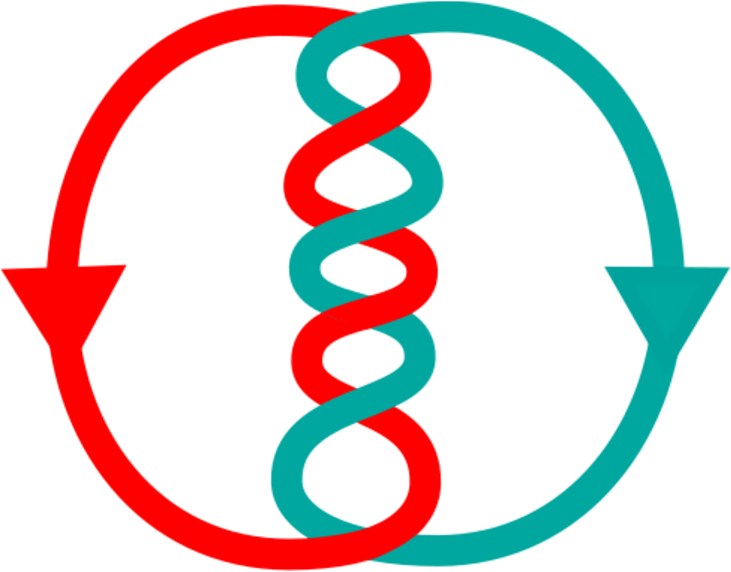
\includegraphics[height=4cm]{images/Gauss_linking_number_002.pdf}}
	\hspace{.125\linewidth}
	\caption{Sketch of two intertwined curves (one in red, one in blue), and their related Gauss linking number}
	\label{fig gauss linking number}
\end{figure}



% ================================================ ENERGY PRINCIPLE ================================================
\subsection{Energy principle}
The ideal MHD equilibrium equations, Eqs.(\ref{equation perp force balance})-(\ref{equation div B ideal mhd}), the Taylor state, Eq.(\ref{equation Taylor state}), and the MRxMHD equilibrium equations, Eqs.(\ref{eq.BeltramiEquation})-(\ref{eq.force_balance}), can be derived from an energy principle. Each derivation is detailed below.

\subsubsection{Ideal MHD} \label{energy principle ideal mhd}
Consider the plasma potential energy, given as the sum of the gas potential energy and the magnetic potential energy, 
\begin{equation}
	W = \iiint_{\mathcal{V}_P} d\mathbf{x}^3 \left(\frac{\mathbf{B}^2}{2} + \frac{p}{\gamma-1}\right), \label{eq. energy functional}
\end{equation}
where $\mathcal{V}_P$ is the plasma volume, $d\mathbf{x}^3$ is a volume element. We now follow \citet{kruskalEquilibriumMagneticallyConfined1958} to minimize $W$ under ideal MHD motions. We assume that the plasma is in an initial state with magnetic surfaces; in general, this initial state will however not be at equilibrium. We now wish to minimize $W$ while conserving the same magnetic topology, \textit{i.e.} conserving the magnetic helicity.

The first step in the derivation is to exploit property of ideal MHD to describe the plasma as a fluid --- a fluid mass element $dm=\rho dv$ is then conserved. Leveraging the ideal gas law, another constant, namely $p^{1/\gamma} / \rho$ is derived. We can thus define the conserved quantity $M(c)$,
\begin{equation}
	M(c) = \int_{\psi_t\leq c} p^{1/\gamma}d\mathbf{x}^3, \label{eq. def M}
\end{equation}
where $c$ is a flux surface label, and $c=C$ is the plasma boundary. Variation of $M$ with respect to $p$ gives
\begin{align}
	0=\delta M &= \frac{1}{\gamma}\int_{\psi_t\leq c} p^{1/\gamma-1}\delta pd\mathbf{x}^3\\
	&=\frac{1}{\gamma}\int_0^c dc \int_{\psi_t=c} p^{1/\gamma-1}\delta p\frac{dS}{|\nabla\psi_t|}, \label{eq. variation M w.r.t p}
\end{align}
while variation of the energy with respect to $p$ gives
\begin{align}
	0=\delta W &= \frac{1}{\gamma-1} \int_0^C dc \int_{\psi_t=c} \frac{dS}{|\nabla\psi_t|}\delta p. \label{eq. variation W w.r.t p}
\end{align}
Both equation (\ref{eq. variation M w.r.t p}) and (\ref{eq. variation W w.r.t p}) have to be satisfied for any variation $\delta p$; in particular, we can choose a variation such that $p^{1/\gamma-1}\delta p/|\nabla \psi_t| = \delta(\mathbf{x}-\mathbf{x}_1)-\delta(\mathbf{x}-\mathbf{x}_2)$, with $\mathbf{x}_i$ a point on the surface $\psi_t=c$. Then equation (\ref{eq. variation M w.r.t p}) is satisfied by construction, and equation (\ref{eq. variation W w.r.t p}) implies
\begin{equation}
	0 = \int_{\psi_t=c}\frac{\delta p}{|\nabla \psi_t|} = \int_{\psi_t=c}\frac{1}{p^{1/\gamma-1}}\delta(\mathbf{x}-\mathbf{x}_1)-\delta(\mathbf{x}-\mathbf{x}_2),
\end{equation}
which is satisfied if $p(\mathbf{x}_1)=p(\mathbf{x}_2)$. Since the $\mathbf{x}_i$ are arbitrary, the pressure must be a function of $c$, \textit{i.e.} $p = p(c)$. Equation (\ref{eq. def M}) can thus be used to express $p(c)$ as
\begin{equation}
	p(c) = \left[\frac{M'(c)}{\int_{\psi_t=c}dS/|\nabla\psi_t|}\right]^\gamma.
\end{equation}

We now express the magnetic field using straight-field line coordinates $(c,\theta_s,\zeta)$ (see appendix \ref{appendix boozer coordinates}) using the Clebsch form,
\begin{equation}
	\mathbf{B} = \nabla\psi_t\times\nabla\nu,
\end{equation}
with
\begin{equation}
	\nu = \lambda(c,\theta,\zeta) + \iotabar\zeta - \theta,
\end{equation}
and $\lambda$ a function that transform arbitrary toroidal coordinates $(c,\theta,\zeta)$ into straight field line coordinates. Variation of the energy function $W$ with respect to $\lambda$ gives
\begin{equation}
	0=\delta W = \int_{\mathcal{V}_P}\mathbf{B}\cdot(\nabla\psi_t\times\nabla\delta\lambda)d\mathbf{x}^3=-\int_{\mathcal{V}_P} \delta\lambda\nabla\cdot(\mathbf{B}\times\nabla\psi_t)d\mathbf{x}^3,
\end{equation}
which implies
\begin{equation}
	\nabla\psi_t\cdot(\nabla\times\mathbf{B})=0,
\end{equation}
\textit{i.e.} magnetic surfaces are current surfaces as well. The final stage of the derivation is to consider variations of $W$ with respect to the toroidal flux. Careful consideration of how the pressure varies as the toroidal flux is varied lead to
\begin{align}
	\int_{\mathcal{V}_P} \delta p(c) \mathbf{x}^3 &= \int_{\mathcal{V}_P}p  \delta \log p\mathbf{x}^3 = \int_0^C dc \int_{\psi_t=c} \frac{dS}{|\nabla\psi_t|} p \gamma \delta\left[\log \left(\frac{M'(c)}{\int dS/|\nabla\psi_t|}\right)\right].
\end{align}
Let us define $I(c)=\int_{\psi_t=c}dS/|\psi_t|$ to lighten the notation. Expanding the variation of the logarithm, we obtain
\begin{align}
	\delta\left[\log\left(\frac{M'(c)}{I(c)}\right)\right] &= \frac{I(c)}{M'(c)} \frac{\delta(M'(c))I(c) - M'(c)\delta(I(c))}{I(c)^2} \\
	&= \frac{\delta(I(c))}{I(c)},
\end{align}
where we used that $M(c)$ is an ideal MHD invariant, \textit{i.e.} $\delta M(c)=0$ and thus $\delta M'(c)=0$. Note that the variation of $I(c)$ can be written as
\begin{equation}
	\delta(I(c)) = \delta\left(\int_{\psi_t=c}\frac{dS}{|\nabla\psi_t|}\right) = \delta \frac{d}{dc}\int_{\mathcal{V}_P}d\mathbf{x}^3 = -\frac{d}{dc}\int_{\psi_t=c}dS\frac{\delta\psi_t}{|\nabla\psi_t|},
\end{equation}
which leads to
\begin{align}
	\int_{\mathcal{V}_P}\delta p(c)d\mathbf{x}^3 &= \gamma\int_0^c dc p(c) \frac{d}{dc}\int_{\psi_t=c}dS\frac{\delta\psi_t}{|\nabla\psi_t|}\\
	&= -\gamma\int_0^c dc p'(c) \int_{\psi_t=c}dS\frac{\delta\psi_t}{|\nabla\psi_t|}\\
	&= -\gamma\int_{\mathcal{V}_P} d\mathbf{x}^3 p'(\psi_t)\delta\psi_t,
\end{align}
where we integrated by part the first equation, and used the assumption that $\delta\psi_t=0$ on the plasma boundary. We can now finally write the variation of the energy,
\begin{align}
	0 = \delta W &= d\mathbf{x}^3 \left[\mathbf{B}\cdot\delta\mathbf{B} + \frac{P'\delta\psi_t + \delta P}{\gamma-1}\right]\\
	&= d\mathbf{x}^3 \left[\mathbf{B}\cdot (\nabla\delta\psi_t\times\nabla\nu + \nabla\psi_t\times\nabla\delta\nu) -P'\delta\psi_t\right]\\
	&= d\mathbf{x}^3 \delta\psi_t\left[(\nabla\times\mathbf{B})\cdot\nabla\nu -p'\right].
\end{align}
To obtain the force balance equation, one needs to take the product between $\nabla\times\mathbf{B}$ and $\mathbf{B}$. We get
\begin{equation}
	\mathbf{B}\times(\nabla\times\mathbf{B}) = [(\nabla\times\mathbf{B})\cdot\nabla\psi_t]\nabla\nu + [(\nabla\times\mathbf{B})\cdot\nabla\nu]\nabla\psi_t = = -p'\nabla\psi_t,
\end{equation}
which is equivalent to
\begin{equation}
	(\nabla\times\mathbf{B})\times\mathbf{B} = \nabla p.
\end{equation}








\subsubsection{Taylor state}
Taylor states do not assume the existence of magnetic surfaces; as a matter of fact, the magnetic helicity is conserved globally, to the opposite of its conservation everywhere in ideal MHD. To enforce this constraint in the energy minimization, we employ the Lagrange multiplier method and minimize the functional
\begin{equation}
	F = \int_{\mathcal{V}_P} \left(\frac{p}{\gamma-1}+\frac{B^2}{2\mu_0}\right)dv - \mu(K-K_0),
\end{equation}
where $K_0$ is the magnetic helicity of the initial state. Variation with respect to $\mu$ enforces the constraint $K=K_0$, while variation with respect to the vector potential $\mathbf{A}$ gives
\begin{align}
	0 = \delta F &= \delta W - \mu(\delta K - K_0)\\
	&= \int_{\mathcal{V}_P} B\delta B dV - \mu \int_V \delta A \cdot B + A \cdot \delta B\\
	&=\int_{\mathcal{V}_P} \left(B \cdot \nabla \times \delta A + A\cdot \delta B - \mu B \cdot \delta A\right) d^3x\\
	&=\int_{\mathcal{V}_P} \left( \nabla \times B - \mu B \right) \cdot \delta Ad^3x + \int_{\mathcal{V}_P}A \cdot \nabla \times \delta A d^3x, \label{eq. taylor state energy 1}
\end{align}
We wish now to prove that the second term of equation (\ref{eq. taylor state energy 1}) vanishes. We write $\nabla\times\delta\mathbf{A}=\delta\mathbf{B}$ and we make use of Faraday's law to write $\delta\mathbf{B} = \nabla\times\mathbf{E}\delta t$ where $\delta t$ is an infinitesimal time over which the plasma motion takes place. We thus get
\begin{align}
	\mathbf{A}\cdot\delta\mathbf{B}&=\left[\nabla\cdot(\mathbf{E}\times\mathbf{A}-\mathbf{E}\cdot\mathbf{B})\right]\delta t\\
	&= \nabla\cdot(\mathbf{E}\times\mathbf{A})\delta t,
\end{align}
where we used Ohm's law (\ref{ideal Ohms law}) to find $\mathbf{E}\cdot\mathbf{B}=0$. Finally, taking the integral over the plasma volume and applying the divergence theorem, we get
\begin{equation}
	\int_{\mathcal{V}_P}A \cdot \nabla \times \delta A d^3x = \int_{\Gamma_{PB}}  (\mathbf{E}\times\mathbf{A})\cdot\mathbf{dS}\delta t = \int_{\Gamma_{PB}}  \mathbf{E}\cdot(\mathbf{A}\times\mathbf{dS})\delta t = 0,
\end{equation}
where we applied the boundary condition $\mathbf{n}\times\mathbf{E}=0$ on the plasma boundary $\Gamma_{PB}$. Equation (\ref{eq. taylor state energy 1}) reduces then to
\begin{equation}
	\int_{\mathcal{V}_P} \left( \nabla \times B - \mu B \right) \cdot \delta Ad^3x = 0,
\end{equation}
which implies the Taylor equilibrium equation (\ref{equation Taylor state}).

\subsubsection{MRxMHD} \label{energy principle mrxmhd}
MRxMHD equations derive as well from an energy principle \citep{Dewar2015}. As described in section \ref{section mrxmhd}, MRxMHD equilibria can be seen as a combination of nested Taylor states at equilibrium with one another. It is thus natural to define the energy functional as the sum of the Taylor's state energy functional relative to each volume, \textit{i.e.}
\begin{equation}
	F = \sum_{l=1}^{N_{vol}} \int_{\mathcal{V}_l} \left[\frac{p}{\gamma-1}+\frac{\mathbf{B^2}}{2\mu_0}\right]d\mathbf{x}^3 + \mu_l(K_l-K_{l,0}). \label{eq.mrxmhd energy functional}
\end{equation}
Minimization with respect to variation in the magnetic field will lead to the Taylor state equation (\ref{eq.BeltramiEquation}) in each volume $\mathcal{V}_l$, while variation with respect to the volume's boundary motion will lead to the equilibrium condition (\ref{eq.force_balance}). The derivation is rather tedious --- further details can be found in the paper by \citet{Dewar2015}.

The ideal MHD, Taylor state and MRxMHD equilibrium equations derive all from an energy principle, as shown in section \ref{energy principle ideal mhd}. This property is leveraged by different numerical codes to find 3D equilibria --- indeed, the equilibrium can directly be computed from an initial state by minimizing an energy functional instead of computing the entire time evolution and trajectory of the plasma. While the time evolution can be of great importance for some applications, it is often a waste of computational time and ressources if only the equilibrium state is sought. For example, the \ac{VMEC} \citep{Hirshman1983,Hirshman1986} finds ideal 3D MHD equilibria by minimizing Eq.(\ref{eq. energy functional}), and the \ac{SPEC} code \citep{hudsonComputationMultiregionRelaxed2012,Hudson2020c} can find MRxMHD equilibrium by minimizing the equation (\ref{eq.mrxmhd energy functional}). The next chapter will focus on describing the \ac{SPEC} code, and how the capability to constraint net toroidal currents has been implemented.




% In MRxMHD, the plasma is divided in $N_{vol}$ nested volumes $\mathcal{V}_l$, so that the MHD energy $W_l$ \citep{kruskal_equilibrium_1958} local to each volume can be written as

% \begin{equation}
% 	W_l = \int_{\mathcal{V}_l} \left(\frac{p_l}{\gamma-1}+\frac{B^2}{2\mu_0}\right)dv,
% \end{equation}
% where $p_l$ is the pressure, $B=|\mathbf{B}|$ is the magnetic field strength, $\mu_0$ is the vacuum permeability, $\gamma$ is the adiabatic constant and $dv$ is an infinitesimal volume element. Minimizing $W$ is then equivalent to minimizing each individual $W_l$. The magnetic helicity is however only constrained to be conserved in each volume $\mathcal{V}_l$ and not everywhere in the plasma. The \ac{MRxMHD} energy functional is then \citep{Hudson2012}

% \begin{equation}
% 	W = \sum_{l=1}^{N_{vol}} \left[W_l -\frac{\mu_l}{2}(K_l-K_{l,0})\right], \label{eq.energy}
% \end{equation}
% where $\mu_l$ is a Lagrange multiplier, $K_l$ is the magnetic helicity in volume $l$ and $K_{l,0}$ the magnetic helicity constraint. The magnetic helicity is defined as 

% \begin{equation}
% 	K_l = \int_{\mathcal{V}_l} \mathbf{A}_l\cdot \mathbf{B}_l dv,
% \end{equation}
% where $\mathbf{A}_l$ is the vector potential of the magnetic field  $\mathbf{B}_l$, \textit{i.e.} $\mathbf{B}_l=\nabla\times\mathbf{A}_l$. In each volume $\mathcal{V}_l$, $l\in\{1,\ldots,N_{vol}\}$, the magnetic field $\mathbf{B}_l$ is varied while keeping the toroidal magnetic flux, $\psi_{t,l}$, and poloidal magnetic flux, $\psi_{p,l}$, constant, until the \ac{MRxMHD} energy (Eq.\ref{eq.energy}) is minimized. The corresponding Euler-Lagrange equations \citep{Hudson2012} describe a force-free magnetic field $\mathbf{B}_l$ satisfying a Beltrami equation,

% \begin{equation}
% 	\nabla\times\mathbf{B}_l = \mu_l\mathbf{B}_l.
% \end{equation}


\end{document}